\documentclass[letterpaper, 11pt, colorful, sections]{jiahua}
\title{Math 1560: Number Theory \textit{Lecture Notes}}
\author{N. Looper}
\date{Spring 2022}

\usepackage[textsize=tiny, textwidth=18mm]{todonotes}
\setuptodonotes{noline, color=green!20}
\usepackage{cancel}
\usetikzlibrary{cd}
\numberwithin{equation}{section}

\begin{document}
\maketitle
\begin{quote}
    \quad These are lecture notes for Math 1560: Number Theory taught at \textsc{Brown University} by Nicole Looper in the Spring of 2022.

    \quad Notes last updated \today.
\end{quote}
\tableofcontents
\bibliographystyle{alpha}
\bibliography{bibliography}

\newpage
%!TEX root = ../notes.tex
\setcounter{section}{-1}
\section{January 27, 2022}
\subsection{Course Logistics}
\begin{itemize}
    \item Mostly refer to syllabus for any information that you might need.
    \item Midterm is planned for March 17.
    \item Final exam schedule can be found on CAB.
\end{itemize}

\subsection{Introduction to Number Theory}
Number theory can be split into two branches: analytic number theory and algebraic number theory.

\emph{What is number theory?} Number theory is the study of integers and their analogues in algebraic number fields.

Prime numbers are a key focus of number theory, and the study of different properties of primes constitutes different fields of number theory:
\begin{enumerate}[i.]
    \item The study of their distributional properties, which is \ul{analytic number theory}.
    \item As building blocks for algebraic numbers, which is \ul{algebraic number theory}.
\end{enumerate}

\subsubsection{Examples of Analytic Number Theory}
Here are some examples of analytic number theory and their statements:
\begin{itemize}
    \item Prime Number Theorem
    \item Twin Prime Conjecture
    \item Goldbach's conjecture
\end{itemize}
\begin{theorem}[Prime Number Theorem]
    Let $\pi(x)$ be the number of primes between $1$ and $x$, then
    \begin{equation*}
        \lim_{x\to\infty} \frac{\pi(x)}{x / \ln(x)} = 1.
    \end{equation*}
\end{theorem}
\begin{conjecture}[Twin Prime Conjecture]
    Twin primes are pairs of primes $p, q$ of the form $q=p+2$. Examples include $(3, 5), (11, 13), \dots$. The conjecture postulates that there are infinitely many twin primes.
\end{conjecture}
\begin{conjecture}[Goldbach's conjecture]
    Any positive even integer greater than $2$ can be written as the sum of $2$ primes.
\end{conjecture}

\subsubsection{Examples of Algebraic Number Theory}
Analyzing the factorization (rings of integers) of number fields is one topic of algebraic number theory.
\begin{example}
    $2$ is prime (irreducible) in $\ZZ$.

    Yet $2$ is not prime in $\ZZ[i]$ (the Gaussian integers). This is because
    \[2 = \underbrace{(1+i)(1-i)}_{\text{associates}}\]
    we have that $(1+i) = i(1-i)$. We also note the property that the principal ideals $(2) = (1+i)^2$ are equal.

    In this example, we say that $2$ ``ramifies'' in the ring of integers.
\end{example}

Fermat's Last Theorem is another such example.

\recall that a \emph{Pythagorean triple} is a triple of the form $a, b, c\in \ZZ_+$ such that
\[a^2 + b^2 = c^2\]
Are there examples of such numbers with different exponents (say, $k^\mathrm{th}$ powers for $k\geq 3$)?
\begin{theorem}[Fermat's Last]
    There are no positive integers $a, b, c\in \ZZ_+$ satisfying
    \[a^k + b^k = c^k\]
    for $k\geq 3$.
\end{theorem}
The answer is no! (Proved by Andrew Wiles)

\begin{conjecture}[$abc$ Conjecture, informally]
    We say \emph{powerful numbers} are positive integers whose prime factorization contains relatively few distinct primes (appropriately weighted) with an exponent of 1.
    \begin{example*}
        $2^{10}3^7$ is powerful, $2^{10}3^{7}5$ is powerful, $1$ is powerful.
    \end{example*}

    If $a, b$ are \emph{very powerful} coprime numbers, then $a+b$ is predicted to be \emph{not powerful}.
\end{conjecture}
\begin{example}
    Consider $2^{10}$ and $3^{15}$. We have
    \[2^{10} + 3^{15} = 14,349,931 = \underbrace{31\cdot 462\cdot 901}_{\text{not powerful}}\]
\end{example}
What about another example, like $3^{15} + 5$? The $abc$ conjecture also predicts that this number is not so powerful...\footnote{After lecture Jiahua: It's a prime!?}
%!TEX root = ../notes.tex
\section{February 1, 2022}
\todo{Happy Lunar New Year! \faHandPeaceO}

\emph{(Thanks Qinan and Andrew for allowing me to shamelessly copy their notes.)}

\subsection{Divisibility and Factorization}
We start with some commonly used notation:
\begin{definition}[Divisibility]
    We use $a\mid b$ to mean ``$a$ divides $b$'' and $a\nmid b$ to mean ``$a$ does not divide $b$''.
\end{definition}

Now for a series of definitions:

\begin{definition}[Primality]
    A positive integer $p\geq 2$ is said to be \ul{prime} if its only positive divisors are $1$ and $p$.
\end{definition}

\begin{definition}[Positive Integers]
    $\ZZ_+$ will denote the \ul{positive integers}.
\end{definition}

\begin{definition}[Order]
    For a nonzero $n\in \ZZ$ and a prime $p$, there is a nonnegative integer $a$ such that $p^a\mid n$ but $p^{a + 1}\nmid n$. This number $a$ is called the \ul{order} of $n$ at $p$, denoted by $\ord_p n$.

    For $n=0$, we set $\ord_p 0 = \infty$. We also have $\ord_p n = 0\Leftrightarrow p\nmid n$.
\end{definition}

We prove a lemma as warm-up:
\begin{lemma}[Existence of Factorization]
    Every nonzero integer can be written as a product of primes.

    \emph{We make an exception for $-1$. The empty product is $1$ so $1$ is fine.}
\end{lemma}
\begin{proof}
    Suppose for the sake of contradiction otherwise, that some nonzero integer can be written as a product of primes. Let $N$ be the smallest integer greater than $2$ that cannot be written as a product of primes.

    $N$ had better not be a prime number itself (since then it would be a product of itself). Then we can write $N = a\cdot b$ where $1 < a, b < N$.

    Since we took $N$ as the least such number that cannot be written as a product of primes, $a$ and $b$ which are less than $N$ can be written as a product of primes. Then $N$ is a product of primes since $a$ and $b$ individually are. This is a contradiction! Thus it had better be the case that \emph{every} nonzero integer can be written as a product of primes.
\end{proof}

This is the theorem we will eventually work toward proving:

\begin{theorem}[Unique Factorization]\label{unique-factorization}
    Every nonzero integer $n$ yields a \emph{unique} prime factorization
    \begin{equation*}
        n = (-1)^\varepsilon\cdot \prod_{p}p^{a(p)}, a(p)\geq 0
    \end{equation*}
    where $\varepsilon = 0$ or $1$, and $\varepsilon, a(p)$ are uniquely determined by $n$. Moreover, we note that $a(p) = \ord_p n$.
\end{theorem}

\subsection{Euclidean and Principal Ideal Domains}
Before this proof, we first recall a conclusion from Math 1530:
\begin{lemma}[Division Lemma]\label{division-lemma}
    If $a, b\in \ZZ$ and $b>0$, then there exists $q, r\in \ZZ$ such that
    \[a = bq + r\]
    with $0\leq r < b$.
\end{lemma}
\begin{proof}
    Consider the set
    \[S = \{a - xb \mid x\in \ZZ\}\]
    We note that $S$ contains \emph{some} positive elements. Let $r = a - qb$ be the least nonnegative element of $S$.

    We claim that $0\leq r < b$. Suppose for the sake of contradiction otherwise, then $r = a - qb \geq b$ gives $a - qb - b \leq 0$ and $a - (q+1)b\leq 0$. Which is a contradiction since we took $r$ to be a the least nonnegative element in $S$ and we've found such smaller element $a - (q+1)b$.

    Then it had better be that $0\leq r < b$ for some $r, q\in\ZZ$.
\end{proof}
\begin{corollary}
    $\ZZ$ is a Euclidean domain, with a Euclidean function given by \cref{division-lemma}.

    $R[x]$ for field $R$ is also a Euclidean domain, with $\lambda = \deg$.
\end{corollary}

\begin{definition}[Euclidean Domain]
    Let $R$ be an integral domain. $R$ is a \ul{Euclidean domain} if there exists a function $\lambda: R\setminus \{0\} \to \NN$ such that if $a, b\in R$ with $b\neq 0$, then there exists some $c, d\in R$ with the property that $a = cb + d$ with $d=0$ or $\lambda(d) < \lambda(b)$.
\end{definition}
\begin{example}
    $\ZZ$ is a Euclidean domain with $\lambda$ function given in \cref{division-lemma}.
\end{example}

\begin{proposition}
    If $R$ is a Euclidean domain, then $R$ is a principal ideal domain. That is, if $I\subseteq R$ is an ideal, then $\exists a\in R$ such that $I = Ra = \{ra\mid r\in R\}$.
\end{proposition}
\begin{proof}
    Assume WLOG that $I$ is not the trivial ideal $I\neq (0)$. Let $0\neq a\in I$ such that $\lambda(a)\leq \lambda(b) \forall b\in I, b\neq 0$.

    We claim that $I = (a) = Ra$.

    We know that $Ra\subseteq I$ since $I$ is an ideal. Let $b\in I$. Then $\exists c, d\in R$ such that $b = ca + d$ where $d = 0$ or $\lambda(d) < \lambda(a)$. Now we have $d = b-ca\in I$, so we can't have $\lambda(d) < \lambda(a)$. Thus $d = 0$, so $b=ca\in Ra$.

    Hence we have $I\subseteq Ra$. Together, we conclude that $I = Ra$.
\end{proof}

\begin{definition}[Principal Ideals, PIDs]
    If $I = (a)$ for some $a\in I$, then $I$ is said to be a \ul{principal ideal}.

    $R$ is a \ul{principal ideal domain} (PID) if every ideal of $R$ is principal.
\end{definition}

Here are some important properties of PIDs:
\begin{enumerate}
    \item Nonunit irreducible elements are exactly the prime elements in $R$.

          \recall $p\in R$ is \ul{irreducible} if $a\mid p\Rightarrow a$ is either a unit or an associate of $p$.

          $p\in R$ is \ul{prime} if $p\mid ab\Rightarrow p\mid a$ or $p\mid b$ and $p$ is a nonzero, nonunit of $R$.

    \item GCDs always exist in PIDs.
\end{enumerate}

\subsection{Unique Prime Factorization}
We're nearly ready to prove unique factorization, after a lemma:
\begin{lemma}\label{additive-orders}
    Suppose $p$ is a prime, and $a, b\in Z$. Then $\ord_p(ab) = \ord_p a + \ord_p b$.
\end{lemma}
\begin{proof}
    WLOG, assume $a, b\neq 0$. We let
    \begin{align*}
        \alpha & = \ord_p a \\
        \beta  & = \ord_p b
    \end{align*}
    Then we have
    \begin{align*}
        a & = p^\alpha\cdot c \text{ where }p\nmid c \\
        b & = p^\beta\cdot d \text{ where }p\nmid d
    \end{align*}
    Thus, $ab = p^{\alpha + \beta}\cdot cd$. We have that $p\nmid cd$ since $p\nmid c$ and $p\nmid d$ (we rely on the fact that if $p$ is irreducible, $p$ is prime). Thus we have that $\ord_p (ab) = \alpha + \beta$.
\end{proof}

\begin{proof}
    (of \cref{unique-factorization}, that $\ZZ$ is a UFD). Recall that for a nonzero $n\in \ZZ$, we write
    \[n = (-1)^\varepsilon \prod_{p}p^a(p), \text{where }\varepsilon = 0\text{ or }1\text{ and }a(p)\geq 0\]
    Given a positive prime $q$, we take $\ord_q$ of both sides. By \cref{additive-orders}, this yields
    \[\ord_q n = \varepsilon\cdot \ord_q (-1) + \sigma_p a(p)\ord_q(p)\]
    Since we have that $\ord_q(-1) = 0$ and $\ord_q(p) = 0, \forall p\neq q$, we've uniquely determined $a(q)$ since $\ord_q(n) = a(q)$. That is, $a(q)$ is \emph{uniquely determined} for all primes $q$. So $n$ has a \emph{unique} prime factorization.
\end{proof}

\subsection{Greatest Common Divisors}
\begin{definition}
    Let $R$ be an integral domain. Then $d\in R$ is said to be a $\gcd$ of two elements $a, b$ if
    \begin{enumerate}[i)]
        \item $d\mid a$ and $d\mid b$,
        \item if $d'\mid a$ and $d'\mid b$, then $d'\mid d$.
    \end{enumerate}
\end{definition}
\begin{remark*}
    An aside for ring theory enthusiasts: $\gcd$ domains are a class of rings mroe general than PIDs or UFDs.
\end{remark*}
We will denote $(a, b)$ as the $\gcd$ of $a$ and $b$.

\textbf{Caution, however!} $\gcd$'s are only unique up to units.

\begin{example*}
    $-5$ and $5$ are both $\gcd$s of $-5$ and $10$ since $-1$ is a unit.
\end{example*}

We will make the convention that the $\gcd$ of 2 integers is the positive $\gcd$, that is, $(-5, 10) = 5$.

An edge case is that $\gcd(0, 0)=0$.

%!TEX root = ../notes.tex
\section{February 3, 2022}

\subsection{Arithmetic Functions}

We look at arithmetic functions and how they act on prime numbers:
\begin{definition}[Arithmetic Function]
    An \ul{arithmetic function} is a function $f: \ZZ_+ \to \CC$.

    \emph{(Typically, these are integer valued.)}
\end{definition}
\begin{example}We have some examples of arithmetic functions:
    \begin{itemize}
        \item Euler $\phi$ function.
        \item $\tau(n)$, the counting function. It takes a positive integer and counts the number of positive divisors of $n$. \[\tau(n) = \sum_{d\mid n} 1\]
        \item $\sigma(n)$, the sum of divisors function. It is the sum over all the positive divisors of $n$. \[\sigma(n) = \sum_{d\mid n}d\]
    \end{itemize}
\end{example}
We have some properties of these functions, like \emph{multiplicative}, \emph{completely multiplicative}, \emph{additive}, \emph{completely additive}.

\begin{definition}[Multiplicativity]
    An arithmetic function $f$ is \ul{multiplicative} if
    \begin{align*}
        f(mn) & = f(m)f(n)\quad \text{whenever }(m, n) = 1
        \intertext{$f$ is said to be \ul{totally or completely multiplicative} if }
        f(mn) & = f(m)f(n)\quad \forall m, n\in\ZZ_+
    \end{align*}
    regardless of coprimality.
\end{definition}

If $f$ is multiplicative and $n_1, \dots, n_k$ are positive pairwise coprime integers, then \[f(n_1\dots n_k) = f(n_1)f(n_2)\dots f(n_k).\]

A particular case that is useful is when we write
\[n=p_1^{e_1}p_2^{e_2}\cdots p_k^{e_k}\]
so that assuming multiplicativity, we have that
\[f(n) = f(p_1^{e_1}) f(p_2^{e_2}) \cdots f(p_k^{e_k})\]
A common type of arithmetic function is a summatory function, namely a function $f$ of the form
\[f(n) = \sum_{d\mid n} g(d), \quad \text{where $g$ is some arithmetic function.}\]

\emph{Food for thought:} how special are summatory functions within the set of all arithmetic functions?

A special property of summatory functions is that they ``inherit multiplicativity''.
\begin{lemma}\label{lemma:summatory-preserves-multiplicativity}
    If $g$ is a multiplicative function, and \[f(n) = \sum_{d\mid n}g(d)\quad \forall n,\] then $f$ itself is multiplicative.
\end{lemma}

\begin{proof}
    Suppose $m, n\in \ZZ_+$ are coprime positive integers.

    The divisors $d$ of $mn$ are the products $a\cdot b$ where $a\mid m$ and $b\mid n$. Each such pair $a, b$ yields a uniquely determined produce $d = a\cdot b$. Conversely, since $(m, n) = 1$, each divisor $d$ of $mn$ determines a unique divisor $a=\gcd(d, m)$ and $b = \gcd(d, n)$ so that $d = a\cdot b$.

    Thus there is a \emph{bijection} between divisors of $mn$ and $m, n$ separately
    \[d\mid mn \longleftrightarrow (a\mid m, b\mid n)\]
    Thus we have
    \begin{align*}
        f(m\cdot n) & = \sum_{d\mid mn}g(d)                                              \\
                    & = \sum_{a\mid m}\sum_{b\mid n}g(ab)                                \\
                    & = \sum_{a\mid m}\sum_{b\mid n}g(a)g(b)                             \\
                    & = \left(\sum_{a\mid m} g(a)\right) \left(\sum_{b\mid n}g(b)\right)
        = f(m)\cdot f(n)
    \end{align*}
    Thus completes the proof that $f$ is multiplicative.
\end{proof}

\recall The functions introduced earlier
\[\tau(n) = \sum_{d\mid n} 1\qquad \sigma(n) = \sum_{d\mid n}d\]
So $\tau$ is the summatory function of the constant $1$ functions, and $\sigma$ is the summatory function of the identity function. We know that the constant $1$ function and the identity function are both completely multiplicative, so $\sigma$ and $\tau$ are multiplicative functions.

The implication of which is that it suffices to apply $\tau$ and $\sigma$ on prime powers and multiply.

Let $p$ be a prime. Then
\begin{align*}
    \tau(p^e)   & = e + 1\quad  \text{(from $p^0$ to $p^e$)}.          \\
    \intertext{We also have}
    \sigma(p^e) & = 1 + p + p^2 + \cdots + p^e = \frac{p^{e+1}-1}{p-1}
\end{align*}
Therefore, if $n=p_1^{e_1}p_2^{e_2}\cdots p_k^{e_k}$, then
\begin{align*}
    \tau(n)   & = \prod_{i=1}^k (e_i + 1)                                 \\
    \sigma(n) & = \prod_{i=1}^k \left(\frac{p_i^{e_i+1}-1}{p_i-1}\right).
\end{align*}
\begin{remark}
    There are higher order divisor functions
    \[\sigma_k(n) = \sum_{d\mid n}d^k\]
    so $\sigma_0 = \tau, \sigma_1 = \sigma, \dots$
\end{remark}

\subsection{Review of \texorpdfstring{$\ZZ/n\ZZ$}{Z/nZ} and its units}

\begin{definition}[Modular Congruence]
    If $a, b, m\in \ZZ$, $m\neq 0$, we say that \ul{$a$ is congruent to $b$ modulo $m$} if $m\mid b-a$. We write
    \begin{equation*}
        a\equiv b\mod{m}, \text{ or more simply } a\equiv b\ (m)
    \end{equation*}
\end{definition}
Congruence mod $m$ is an equivalence relation on $\ZZ$. If $a\in \ZZ$, $\overline{a}$ denotes the set of integers congruent to $a\mod m$, i.e. $\overline{a} = \{a + km \mid k\in \ZZ\}$.

\begin{definition}[$\ZZ/m\ZZ$, Residues mod $m$]
    The set of congruence classes mod $m$ is denoted $\ZZ/m\ZZ$. This is a quotient ring of the ring of integers $\ZZ$.

    If $\overline{a}_1, \overline{a}_2, \dots, \overline{a}_m$ form a complete set of congruence classes mod $m$, then the set of integers $\{a_1, a_2, \dots, a_m\}$ is called a \ul{complete set of residues mod $m$}.
\end{definition}

$\ZZ/m\ZZ$ can be endowed with the structure of a commutative ring by setting
\begin{align*}
    \overline{a} + \overline{b}               & = \overline{a + b} \\
    \text{and }\overline{a}\cdot \overline{b} & = \overline{ab},
\end{align*}
and proving that this is well-defined as ring operations.

\begin{proposition}
    The set of units in $\ZZ/m\ZZ$ is exactly
    \[\{\overline{a}\mid (a, m) = 1\}\]
\end{proposition}
\begin{proof}
    Let $\overline{a}\in \ZZ/m\ZZ$, then
    \begin{align*}
                              & \exists \overline{b}\in \ZZ/m\ZZ\text{ s.t. }\overline{b}\cdot \overline{a}\equiv 1\mod m \\
        \Longleftrightarrow\  & \exists b, n\in \ZZ\text{ s.t. } ba - mn = 1                                              \\
        \intertext{Then by B\'ezout's identity...}
        \Longleftrightarrow\  & (a, m) = 1
    \end{align*}
\end{proof}

\subsection{The Euler \texorpdfstring{$\phi$}{phi} Function}
For $n\in \ZZ_+$, $\phi(n)$ is defined to be the number of integers $1\leq m\leq n$ coprime to $n$.
\begin{example}
    We have some examples of the Euler $\phi$ functions:
    \begin{align*}
        \phi(1)   & = 1                                                                 \\
        \phi(p)   & = p-1 \text{ for any prime $p$}
        \intertext{Let $e\geq 1$, }
        \phi(p^e) & = p^e-p^{e-1} \text{ for prime powers, we exclude multiples of $p$}
    \end{align*}
\end{example}

\emph{Wouldn't be great if $\phi$ were multiplicative? It is!}
\begin{theorem}
    If $(m,n) = 1$, then $\phi(mn) = \phi(m)\phi(n)$.
\end{theorem}
\begin{proof}
    By the Chinese Remainder Theorem\footnote{This is an easy way to prove this assuming Math 1530 (Abstract Algebra). There is another way to prove this with one hand tied behind the back, it just takes more mental muscle to do. }, $\ZZ/mn\ZZ\cong \ZZ/m\ZZ\times \ZZ/n\ZZ$ if $(m, n) = 1$.

    Taking the unit groups on both sides, we have
    \[(\ZZ/mn\ZZ)^\times \cong (\ZZ/m\ZZ)^\times \times (\ZZ/n\ZZ)^\times\]
    and the Euler $\phi$ function is simply measuring the order of said unit groups ($\phi(n) = \left|(\ZZ/n\ZZ)^\times\right|$).
\end{proof}

Here is an important fact about the Euler $\phi$ function:
\begin{proposition}
    We have
    \begin{equation*}
        \sum_{d\mid n}\phi(d) = n.
    \end{equation*}
\end{proposition}
\begin{proof}\emph{(1: a cute, snazzy proof)}
    Consider the $n$ rational numbers
    \[\frac{1}{n}, \frac{2}{n}, \dots, \frac{n-1}{n}, \frac{n}{n} = 1\]
    and reduce all to lowest terms so that the numerator and denominator are coprime.

    Q: Given a positive divisor $d$ of $n$, how many fractions have $d$ as the denominator?

    A: We have exactly $\phi(d)$ of them.

    Conversely, every denominator $d$ is certainly a divisor of $n$. So we conclude that $\displaystyle n = \sum_{d\mid n}\phi(d)$.
\end{proof}
\begin{proof}\emph{(2: using what we've learnt)}
    We use the fact that $\phi$ is multiplicative, and that this function is a summatory function of $\phi$, so this function itself is multiplicative. We can decompose this into prime powers. So it suffices to show this for prime powers.

    Let $n = p^k$. Let
    \[f(n) = \sum_[d\mid n]\phi(d).\]
    Then we have
    \begin{align*}
        f(p^k) = \sum_{d\mid p^k} \phi(d) & = 1 + (p-1) + (p^2 - p) + \dots + (p^k-p^{k-1})
        \intertext{which is a telescoping sum which leaves}
                                          & = p^k
    \end{align*}
    which is as intended. 
\end{proof}
%!TEX root = ../notes.tex
\section{February 8, 2022}

\subsection{Dirichlet Convolutions}

\begin{definition}[Dirichlet Convolution]
    Let $f, g$ be arithmetic functions. Then the \ul{Dirichlet convolution/product} of $g$ and $g$ it
    \begin{align*}
        (f * g)(n) : & = \sum_{d_1d_2=n}f(d_1)g(d_2) \\
                     & = \sum_{d\mid n}f(d) g(n/d)
    \end{align*}
\end{definition}

We do check that this has properties that we want it to have, like associativity:
\begin{align*}
    ((f * g) * h)(n) & = (f * (g * h))(n)                      \\
                     & = \sum_{d_1d_2d_3=n} f(d_1)g(d_2)h(d_3)
\end{align*}
It is also clearly commutative.

We also have that this product has a multiplicative identity.

\begin{definition}
    Let $I : \ZZ_+\to \{0, 1\}$ be given by
    \[I(n) = \begin{cases}
            1 & \text{if } n = 1 \\
            0 & \text{otherwise}
        \end{cases}\]
    Then $I$ is an identity for $*$, in the sense that $f * I = I * f = f$.
\end{definition}

\begin{lemma}
    If $f$ is an arithmetic function such that $f(1)\neq 0$, then there exists an arithmetic function $g$ such that $f * g = I$.

    It is given recursively by
    \begin{align*}
        g(1) & = \frac{1}{f(1)}                                         \\
        g(n) & = -\frac{1}{f(1)}\cdot \sum_{d\mid n, d < n} g(d) f(n/d)
    \end{align*}
\end{lemma}
\begin{proof}
    We want to show that given $g$ and $g$ defined as above, we have that $f * g = I$.

    $n=1$: \[g(1)\cdot f(1) = \frac{1}{f(1)}f(1) = 1\]

    $n > 1$: \begin{align*}
        \sum_{d\mid n}g(d) f(n/d) & = g(n)\cdot f(1) + \sum_{d\mid n, n<n}g(d) f(n/d)                   \\
                                  & = -\frac{1}{f(1)}\cdot \sum_{d\mid n, d < n} g(d) f(n/d) \cdot f(1)
        + \sum_{d\mid n, n<n}g(d) f(n/d)                                                                \\
                                  & = 0
    \end{align*}
    So $g$ is indeed an inverse of $f$ since they produce the identity function $I$.
\end{proof}

\subsection{M\"obius Inversion}
The motivation of this is: given a summatory function of multiplicative functions, can we recover the multiplicative function?
\begin{definition}[M\"obius $\mu$ Function]
    We define $\mu : \ZZ_+ \to \{-1, 0, 1\}$ given by
    \[\mu(n) = \begin{cases}
            (-1)^k & \text{if $n = p_1p_2\dots p_k$ if $p_i$ are pairwise distinct primes} \\
            0      & \text{otherwise}
        \end{cases}\]
    \emph{(We note that $\mu(1) = 1$.)}
\end{definition}

\begin{lemma}
    $\mu$ is a multiplicative function.
\end{lemma}
\begin{proof}
    Let $m, n\in\ZZ_+$ such that $(m, n) = 1$. We write
    \begin{align*}
        m & = p_1^{e_1}p_2^{e_2}\cdots p_k^{e_k} \\
        n & = q_1^{f_1}q_2^{f_2}\cdots q_l^{f_l} \\
    \end{align*}
    \begin{description}
        \item[Case 1]
            Some exponent $e_i$ or $f_i \geq 2$. Then we have that \[\mu(mn) = \mu(m)\mu(n) = 0\]
        \item[Case 2]
            We have that \begin{align*}
                m & =p_1p_2\cdots p_k \\
                n & =q_1q_2\cdots q_l
            \end{align*}
            where $p_i$ and $q_i$ are all pairwise distinct. Then $\mu(m) = (-1)^k$ and $\mu(n) = (-1)^l$, so $\mu(m) = \mu(n) = (-1)^{k+l}$.

            Since these are coprime $(m, n) = 1$, then we have that $\mu(mn) = (-1)^{k+l}$.
    \end{description}
    Which is as intended, giving that $\mu$ is a multiplicative function.
\end{proof}

\begin{lemma}
    We have the property:
    \begin{align*}
        \sum_{d\mid n}\mu(d) = 0 \qquad \forall n\geq 2.
    \end{align*}
    Which tells us that the summatory function of $\mu$ is $I$.
\end{lemma}
\begin{proof}
    We define
    \begin{align*}
        f(n) := \sum_{d\mid n}\mu(d) \qquad \text{is multiplicative}
    \end{align*}
    We check this on prime powers, for prime $p$ and $e\geq 1$:
    \begin{align*}
        f(p^e) & = \mu(1) + \mu(p) + \mu(p^2) + \cdots + \mu(p^e) \\
               & = 1 - 1 + 0 + \cdots + 0 = 0
    \end{align*}
    so we're done since $f$ is multiplicative and is $0$ for all power of primes.
\end{proof}

\begin{lemma}
    Let $i: \ZZ_+\to \{1\}$ be the constant $1$ function.
    \[i * \mu = \mu * i = I\]
\end{lemma}
\begin{proof} In the case of $n=1$, we have $i(1)\mu(1) = 1$.

    For $n > 1$, we have $(i * \mu)(n) = \displaystyle \sum_{d\mid n}\mu(d) = 0$ from above.
\end{proof}

We see here that summatory functions can be seen as Dirichlet products: the summatory function $F$ of $f$ is $F = f * i$. What we said about summatory functions being multiplicative boils down to Dirichlet convolutions preserving multiplicativity.

\recall that summatory functions inherit multiplicativity. In fact, this holds for Dirichlet products as well. If $f, g$ are multiplicative, then so is $f * g$.

The proof is parallel to the proof for summatory functions, for \cref{lemma:summatory-preserves-multiplicativity}.

\begin{theorem}[M\"obius Inversion]
    Let
    \begin{align*}
        F(n) & = \sum_{d\mid n} f(d)                         \\
        \intertext{Then we have }
        f(n) & = \sum_{d\mid n}\mu(d)\cdot F(n/d) = \mu * F.
    \end{align*}
\end{theorem}
\begin{proof}
    $F = f * i$, then \[F * \mu = (f * i) * \mu = f * (i * \mu) = f * I = f.\]
    which was simpler than I expected\dots
\end{proof}

\begin{corollary}\label{cor:summatory-multiplicativity-original-multiplicative}
    If $F$ is the summatory function of $f$, and $F$ is multiplicative, then $f$ is also multiplicative, as $f = \mu * F$ and $\mu$ is multiplicative and convolutions with multiplicative functions are multiplicative.
\end{corollary}
\begin{corollary}
    \Cref{cor:summatory-multiplicativity-original-multiplicative} gives another proof that $\phi$ is multiplicative, as \[\sum_{d\mid n}\phi(d) = \phi * i = \mathrm{id}.\]
\end{corollary}

\subsection{Applications of M\"obius Inversion}
\subsubsection{Cyclotomic Polynomials}

\recall the $n^\mathrm{th}$ cyclotomic polynomial $\Phi_n(x)$ is the unique irreducible polynomial in $\ZZ[x]$ dividing $x^n - 1$ but no $x^k - 1$ for $k < n$.

Thus \[\Phi_n(x) = \prod_{\substack{1\leq k < n \\ (k, n) = 1}} \left(x - e^{2\pi i k / n}\right)\]
as the roots of this polynomial are exactly the primitive $n^\mathrm{th}$ roots of unity. We have that \[\prod_{d\mid n}\Phi_d(x) = x^n - 1.\]
By M\"obius inversion, if
\begin{align*}
    G(n) & = \prod_{d\mid n}g(d),
    \intertext{then we have that}
    g(n) & = \prod_{d\mid n}G(d)^{\mu(n/d)}
\end{align*}
In particular, taking $G(n) = x^n - 1$ (with particular $x\in\CC$) as an arithmetic function, we have \[\Phi_n(x) = \prod_{d\mid n}(x^d - 1)^{\mu(n/d)}\qquad (x\in \CC)\]
Applying this identity for enough $x\in \CC$ yields this as an identity of polynomials.

\subsubsection{Dynatomic Polynomials}
The roots of cyclatomic polynomials are roots of unity. Dynatomic polynomials have as roots the periodic points (of certain periods) of a polynomial.

\begin{definition}
    Let $K$ be a field, and let $f\in K[x]$ of degree $d\geq 2$. Let \[f^n = \underbrace{f\circ f\circ \cdots \circ f}_{n\text{ times}}\]
    then $P\in \overline{K}$\footnote{Algebraic numbers in field $K$, the field you get by adjoining all roots of polynomials in $K[x]$.} is said to be \ul{periodic} under $f$ if
    \[f^n(P) = P\qquad \text{for some $n\geq 1$}\]
\end{definition}
\begin{example}
    Let $f(x) = x^2 - 1$. $0$ is a period point under $f$:
    \[0\longmapsto -1\longmapsto 0\]
    and its \ul{period} is $2$.

    \begin{remark*}
        If $n$ is the smallest positive integer such that $f^n(p) = p$ ($p$ periodic), then we call $n$ the \ul{exact period} of $p$ under $f$.
    \end{remark*}
\end{example}
\begin{definition}
    The $n^\mathrm{th}$ dynatomic polynomial of $f$ is 
    \[\Phi_{f,n}(x) := \prod_{d\mid n}\left(f^d(x) - x\right)^{\mu(n/d)}\]
\end{definition}
We hope that $\Phi_{f, n}(x)$ has as its roots the points of exact period $n$\dots This hope is dashed\dots 
\begin{example}
    $f(x) = x^2 - \frac{3}{4}$. 
    \begin{align*}
        f^2(x) - x &= \left(x - \frac{3}{2}\right)\left(1 - \frac{1}{2}\right)^3 \\
        f(x) - x &= \left(x-\frac{3}{2}\right)\left(x + \frac{1}{2}\right)
    \end{align*}
    Thus \[\frac{f^2(x) - x}{f(x) - x} = \left(x + \frac{1}{2}\right)^2\]
    But $x=-\frac{1}{2}$ is \ul{fixed} under $f$. 
\end{example}
%!TEX root = ../notes.tex
\section{February 10, 2022}

\subsection{Congruences \emph{continued}}
\recall that for $m\in\ZZ_+$, $a,b\in \ZZ$, the linear congruence
\[ax\equiv b\mod{m}\]
has a solution if and only if $(a, m)\mid b$. Unwinding this gives Bezout's identity.

\textbf{Q: How do we actually find a solution?}

\textbf{A:} Either guess and check; or apply the following algorithm:
\begin{enumerate}[1)]
    \item Divide all terms in the congruence by $d = (a, m)$.
    \item If step $1$ yields
          \[a'x\equiv b'\mod m'\]
          with $(a', m') = 1$, then $d:= (a', b')$ is a \ul{unit} mod $m'$, so we can divide both sides by $d'$.
          \[a'd'^{-1}x\equiv b'd'^{-1}\mod m'\]
    \item Let $a''x\equiv b''\mod m$ be the result so far. We replace $b''$ by some $b''+km'$\footnote{Since made $a'$ and $m'$ coprime, we have $(a', m')=1$ so we can indeed solve congruence $a''q \equiv b''+km'$ gives noncoprime pairs.} such that $(a'', b''+km')>1$ allows us to repeat step $2$. This results in some $a'''$ such that $|a'''| < |a''|$.

          Given that we repeat this process, this must eventually terminate, since the absolute values of the $a$ terms are strictly decreasing each time.
\end{enumerate}
\begin{example}
    Let $10x\equiv 6\mod{14}$.

    \begin{enumerate}[1)]
        \item $(a, m) = (10, 14) = 2$ so we divide through by $2$. \[5x\equiv 3\mod{7}\]
        \item Irrelevant since $(5, 3)$ are coprime.
        \item Consider integers of form $3+7k$, and see which are divisible by $5$. We can take $k=1$. We get
              \[5x\equiv 10\mod 7\]
        \item[2)] Divide by $(5, 10) = 5$ so we have $x\equiv 2\mod{7}$.
    \end{enumerate}
\end{example}

\subsection{Simultaneous Linear Congruences}
\recall the CRT/Sun-tzu's theorem.
\begin{theorem}[Sun-tzu's Theorem / Chinese Remainder Theorem]
    Suppose that $m = m_1m_2\cdots m_t$ with $(m_i, m_j) = 1 \forall i\neq j$.

    Let $b_1, b_2\dots, b_t$ be integers, and consider the system of congruences
    \begin{align}
        x_1 & \equiv b_1\mod{m_1}        \label{eqn:crt-congruences} \tag{$*$} \\
        x_2 & \equiv b_2\mod{m_2} \nonumber                                    \\
            & \qquad \vdots \nonumber                                          \\
        x_t & \equiv b_t\mod{m_t} \nonumber
    \end{align}
    Then this system has a unique solution modulo $m$\footnote{That is, we have at least one solution, and we can shift it by \emph{any} multiple of $m$.}.
\end{theorem}
\begin{proof}
    Let $n_i = m_1m_2\cdots \cancel{m_i}\cdots m_t = \frac{m}{m_i}$ for each $i$. Since $m_i$ is coprime to $m_j,\ \forall j\neq i$, we have $(n_i, m_i) = 1 \forall i$. Then, there exists solutions $r_i, s_i\in \ZZ$ such that
    \[r_im_i + s_in_i = 1\]
    Let $e_i = s_in_i$. Then for each $i$,
    \[e_i\equiv 1\mod m_i\]
    and $e_i\equiv 0\mod m_j,\ \forall j\neq i$.

    Our goal is to ultimately show
    \[\ZZ/m\ZZ\simeq \ZZ/m_1\ZZ\times \ZZ/m_2\ZZ\times\cdots\times\ZZ/m_t\ZZ\]
    with each $e_i$ generating the ``$\ZZ/m_i\ZZ$ piece''.

    Set \[x_0 = \sum_{i=1}^t b_ie_i\] so that $x_0\equiv b_i\pmod{m_i}\ \forall i$, so $x_0$ is a solution to \cref{eqn:crt-congruences}.

    Suppose $x_1$ is another solution. Then we have
    \[x_1-x_0\equiv 0\mod{m_i}\ \forall i, 1\leq i\leq t\]
    Since the $m_i$ are pairwise coprime, we get $m\mid x_1-x_0$.
\end{proof}

\subsection{Structure of Unit Groups}
\recall in Math 1530, we learned Lagrange's theorem
\begin{theorem}[Lagrange's Theorem]
    If $G$ is a finite group, then for every subgroup $H$ of $G$, we have $|H| \bigm\vert |G|$.
\end{theorem}
\begin{corollary}
    If $G$ is a finite group of order $n$, and $a\in G$, then $a^n = e$, where $e$ is the identity of the group.
\end{corollary}
We've seen that $\left\vert U(m) \right\vert = \phi(m)$.\footnote{For notation, we use $U(m) := (\ZZ/m\ZZ)^\times$.} Applying Lagrange's theorem, we have Euler's theorem:
\begin{theorem}[Euler's Theorem]\label{thm:eulers-thm}
    For any $a\in \ZZ$ with $(a, m) = 1$, we have $a^{\phi(m)}\equiv 1\mod{m}$.
\end{theorem}
\begin{definition}
    A subset $R$ of $\ZZ$ is said to be a \ul{reduced set of residues mod $m$} if $R$ contains exactly one element from each of the $\phi(m)$ congruence classes that are units mod $m$.
\end{definition}
\begin{proof}[Alternate proof of \cref{thm:eulers-thm}]
    Let $R = \{r_1, r_2, \dots, r_{\phi(m)}\}$ be a reduced set of residues mod $m$. If $(a, m) = 1$, then $aR$ is also a reduced set of residues mod $m$. Thus, if $x_1, x_2, \dots, x_{\phi(m)}\in aR$ (pairwise distinct), then
    \begin{align*}
        x_1x_2\cdots x_{\phi(m)}               & \equiv r_1r_2\cdots r_{\phi(m)}\mod{m}  \\
        (ar_1)(ar_2)\cdots (ar_{\phi(m)})      & \equiv r_1r_2\cdots r_{\phi(m)}\mod{m}  \\
        a^{\phi(m)} (r_1r_2\cdots r_{\phi(m)}) & \equiv r_1r_2\cdots r_{\phi(m)} \mod{m} \\
        \intertext{since all the $r_i$ are units mod $m$, we divide through}
        a^{\phi(m)}                            & \equiv 1\mod{m}
    \end{align*}
    Which is as desired.
\end{proof}

We'll be studying roots of polynomials over $\ZZ/m\ZZ$, especially polynomials of the form $x^d - a$.

By Sun-tzu's theorem, the case of $m$ being a prime power is especially important. This turns out to have a lot to do with the case that $m=p$ is a prime itself.

First something further \emph{afield}:
\begin{proposition}\label{prop:d-roots-in-fp}
    If $p$ is a prime and $p\nmid d$ for $d\in\ZZ_+$, then the polynomial
    \[x^d - a\in (\ZZ/p\ZZ)[x],\qquad a\not\equiv 0\mod{p}\]
    has exactly $d$ roots in some extension of $\FF_p$.

    Conversely, if $p\mid d$, then there are fewer than $d$ roots in any extension of $\FF_p = \ZZ/p\ZZ$.
\end{proposition}

The proof uses the following proposition:
\begin{proposition*}
    A nonzero polynomial $f\in K[x]$ is \ul{separable} if and only if it is relatively prime to its derivative $f'$. (A separable polynomial whose roots in its algebraic closure $\overline{K}$ whose roots are all distinct).
\end{proposition*}
\begin{proof}
    ~\begin{description}
        \item[$\Rightarrow$ Right Direction:]
            Suppose $f$ is separable and $\alpha$ be any root of $f$. Then $f(x) = (x-\alpha)h(x)$, where $h(\alpha)\neq 0$ since $\alpha$ is a non-repeated root.

            We have $f'(\alpha) = h(\alpha)\neq 0$, so $\alpha$ is not a root of $f'$. Thus $f$ and $f'$ have no common roots, so they are coprime.

        \item[$\Leftarrow$ Left Direction:]
            Prove by contrapositive. Suppose $f$ is not separable. i.e. it has some repeated root which we call $\alpha$.

            Then $f(x) = (x-\alpha)^2g(x)$, so $f'(x) = (x-\alpha)^2 g'(x) + 2(x-\alpha)g(x)$. We see that $x-\alpha$ divides both $f$ and $f'$ so $(f, f')\neq 1$.
    \end{description}
    Which concludes the bidirectional.
\end{proof}
\begin{proof}[Proof of \cref{prop:d-roots-in-fp}]
    We have $f(x) = x^d - a$, $a\not\equiv 0\pmod{p}$ has $d$ distinct solutions in some extension of $\FF_p = \ZZ/p\ZZ$, because \[f'(x) = dx^{d-1}\pmod{p}\] and with $0$ as its only root but $0$ is not a root of $f$. By above we have that $f$ is separable.

    Conversely, if $p\mid d$, then
    \[f'(x)\equiv 0\pmod{p},\]
    so $(f, f')\neq 1$, meaning that $f$ is not separable.
\end{proof}

\begin{proposition}[4.1.2 of text]\label{prop:d-roots}
    If $p$ is a prime and if $d\mid p-1$, then the polynomial
    \[x^{d-1}\in (\ZZ/p\ZZ)[x]\] has exactly $d$ roots in the base field $\FF_p = \ZZ/p\ZZ$.
\end{proposition}
\begin{proof}
    We know this is true in the case of $d = p-1$ because of Fermat's Little Theorem (also Euler's Theorem).

    We also note that $(x^d - 1)\mid (x^{p-1} - 1)$. Since $x^{p-1} - 1$ has all roots in the base field by FLT, $x^d - 1$ had better also retain its roots in the base field $\FF_p$ by contradiction.
\end{proof}
%!TEX root = ../notes.tex
\section{February 15, 2022}

\subsection{Cyclicity of Groups}
\subsubsection{mod odd \texorpdfstring{$p$}{p}}
\recall from last class, we had \cref{prop:d-roots}:
\begin{proposition*}
    If $p$ is a prime and if $d\mid p-1$, then the polynomial
    \[x^{d-1}\in (\ZZ/p\ZZ)[x]\] has exactly $d$ roots in the base field $\FF_p = \ZZ/p\ZZ$.
\end{proposition*}
\begin{corollary}\label{cor:generators-in-p}
    $G:=(\ZZ/p\ZZ)^\times$ is cyclic.
\end{corollary}
\begin{proof}
    For $d\mid (p-1)$, we write $\psi(d)$ for the number of elements of $G$ having order $d$.

    Proposition 2 implies that\footnote{We throw in Lagrange's theorem, and essentially count the number of solutions to $x^d\equiv 1$.}
    \[\sum_{c\mid d}\psi(c) = d\qquad(\psi* i = \id, \psi = \id * \mu)\]
    M\"obius inversion gives
    \[\psi(d) = \sum_{c\mid d}\mu(c)\frac{d}{c}.\]
    On the other hand, we have $\id = \phi * i\Rightarrow \phi = \mu * \id$. Thus $\psi(d) = \phi(d)$ for all $d\mid (p-1)$.
    So in particular, $\psi(p-1) = \phi(p-1)\geq 1$ for any prime $p$.
\end{proof}

\subsubsection{mod odd power \texorpdfstring{$p^e$}{p\^e}}
\begin{theorem}\label{thm:generators-in-powers-of-p}
    Let $p\in \ZZ_+$ be an odd prime, and let $e\geq 1$. Then $U(p^e)$ is cyclic.
\end{theorem}
Proof overview:
\begin{enumerate}[1.]
    \item Pick a primitive root mod $p$. We call it $g$ (for generator).
    \item Show that either $g$ or $g + p$ is a primitive root mod $p^2$.
    \item Show that if $h$ is any primitive root mod $p^2$, then $h$ is a primitive root mod $p^e$ $\forall e\geq 2$.
\end{enumerate}
\begin{proof}[Proof of \cref{thm:generators-in-powers-of-p}]
    ~\begin{description}
        \item[Step 1.] Let $g$ be a primitive root modulo $p$ given by \cref{cor:generators-in-p}.
        \item[Step 2.]  Let $d$ be the order of $g$ mod $p^2$. Since $\phi(p^2) = p(p-1)$, we have that
            \[d\mid p(p-1)\qquad\text{by Lagange}.\]
            By definition of $d$,
            \begin{align*}
                g^d\equiv 1\mod{p^2}
                \intertext{so we also have}
                g^d\equiv 1\mod{p}
            \end{align*}
            Thus $(p-1)\mid d$ since $g$ has order $p-1$ mod $p$. Altogether, $d$ is either $p-1$ or $p(p-1)$. If $d = p(p-1)$, then we are done with step 2. So we assume the former that $d = p-1$.

            Let $h = g + p$. We know that $h$ is a primitive root mod $p$, so we do the same [yoga] as above and conclude that the order of $h$ mod $p^2$ is either $p-1$ or $p(p-1)$.

            By our new hypothesis,
            \[g^{p-1}\equiv 1\pmod{p^2}\]
            so modulo $p^2$, we have
            \begin{align*}
                h^{p-1} = (g+p)^{p-1} & = g^{p-1} + (p-1)g^{p-2}p + \cdots + p^{p-1}
                \intertext{Modulo $p^2$, the only terms that survive are (expand and all $p^2$ terms die):}
                                      & \equiv 1 - pg^{p-2}\pmod{p^2}
            \end{align*}
            But $p\nmid g$, so $pg^{p-2}\not\equiv 0\mod{p}$, and hence $h^{p-1}\not\equiv 1\mod{p^2}$. Thus the order of $h$ mod $p^2$ is $p(p-1)$, so $h$ generates $U(p^2)$.

            So we are done with step $2$. If $g$ is a primitive root mod $p$, then either $g$ or $g + p$ is a primitive root mod $p^2$.
        \item[Step 3.] We wish to show that a primitive root mod $p^2$ is also a primitive root mod $p^e$ $\forall e\geq 2$. We induct on $e$.

            Let $h$ be a primitive root mod $p^e$ for some fixed $e\geq 2$. Let $d$ be the order of $h$ mod $p^{e+1}$. By Lagange, we have that $d\mid \phi(p^{e+1}) = p^e(p-1)$, and from step $2$,
            \[\phi(p^e) = p^{e-1}(p-1)\mid d\]
            Hence $d = p^e(p-1)$ or $p^{e-1}(p-1)$. If it's the former then we are done, so we assume latter.

            We want to show that
            \[h^{p^{e-1}(p-1)}\not\equiv 1\mod{p^{e+1}}\]
            implying that $d = p^e(p-1)$ after all.

            Since $h$ has order $\phi(p^e) = p^{e-1}(p-1)$ in $U(p^e)$, we have \begin{equation}
                h^{p^{e-2}(p-1)}\not\equiv 1\mod{p^e} \label{eqn:5.2-1}\tag{$\star$}
            \end{equation} However,
            \begin{equation}
                h^{p^{e-2}(p-1)}\equiv 1\mod{p^{e-1}} \label{eqn:5.2-2}\tag{$\star\star$}
            \end{equation}
            Combining \cref{eqn:5.2-1} and \cref{eqn:5.2-2} yields
            \[h^{p^{e-2}(p-1)}=1+kp^{e-1}\]
            where $p\nmid k$. Therefore, we have
            \begin{align*}
                h^{p^{e-1}(p-1)} & = (1+kp^{e-1})^p                                    \\
                                 & = 1 + pkp^{e-1} + \binom{p}{2}k^2p^{2e-2} + \cdots
                \intertext{Subsequent terms are all divisible by $p^{3e-3}=(p^{e-1})^3$, and hence divisible by $p^{e+1}$ as $e(e-1)\geq 2+1\ \forall e\geq 2$. Thus
                }
                h^{p^{e-1}(p-1)} & = 1 + kp^e + \frac{1}{2}k^2p^{2e-1}(p-1)\mod{p^e+1}
            \end{align*}
            $p$ is odd, so
            \[\frac{1}{2}k^2p^{2e-1}(p-1)\]
            is divisible by $p^{e+1}$, since $2e-1\geq e+1$. Thus
            \[h^{p^{e-1}(p-1)} \equiv 1 + kp^e \mod{p^e+1}\]
            Since $p\nmid k$, we get that $kp^e\not\equiv 0$ so
            \[h^{p^{e-1}(p-1)} \not\equiv 1 \mod{p^e+1}\]
            This proves that $d = p^e(p-1)$, which is to say that $h$ is a primitive root mod $p^{e+1}$.
    \end{description}
    Altogether, we have that $U(p^e)$ is cyclic.
\end{proof}

\subsubsection{mod powers of 2}
\begin{theorem}
    $U(2^e)$ is cyclic iff $e = 1$ or $e = 2$.
\end{theorem}
\begin{proof}
    Clearly $U(2)$ and $U(4)$ are cyclic\footnote{We don't have much choice since there is only one trivial group and one group of order $2$, both cyclic.}.

    We show that $U(2^e)$ is \emph{not} cyclic for all $e\geq 3$. Notice: it suffices to show that $U(8)$ is not cyclic, since we can find group homomorphisms down powers of $2$.
    \[U(8) = \{\overline{1}, \overline{3}, \overline{5}, \overline{7}\}\]
    and $\overline{1}^2 = \overline{3}^2 = \overline{5}^2 = \overline{7}^2\mod{8}$.
\end{proof}

\subsection{Classification of all cyclic unit groups}
\begin{corollary}
    $U(m)$ is cyclic if and only if $m = 1, 2, 4, p^e$ or $2p^e$ for some odd prime $p$.
\end{corollary}
\begin{proof}
    Recall that a product $G$ of finite cyclic groups $G_1$ and $G_2$ is cyclic iff $(|G_1|, |G_2|) = 1$.\footnote{Secretly, Chinese Remainder Theorem.} On the other hand, $\phi(m)$ is even $\forall m\geq 3$. So only one of $G_1$ and $G_2$ needs odd power.

    Combined with our structure theorems on $U(p^e)$ for primes $p$, this proves the corollary since these are the only possibilities.
\end{proof}
%!TEX root = ../notes.tex
\section{February 17, 2022}
\subsection{Special Integers}
\subsubsection{Fermat and Mersenne Primes}
We make the observation that many small primes are of the form $2^m\pm 1$ for some natural number m, for example
\[3, 5, 7, 17, 31\]
We deal with the $+1$ and $-1$ cases separately.
\begin{lemma}
	If $2^m + 1$ is prime, then $m = 2^n$ for some $n\geq 0$.
\end{lemma}
\begin{proof}
	We show the contrapositive. Suppose $m$ is not a power of $2$. We write $m=2^n\cdot q$ for some odd $q>1$.

	The polynomial
	\[f(t) = t^q + 1\]
	has $t=-1$ as a root, so
	\[f(t) = (t+1)g(t) \quad \text{where $\deg f = q > 1$}\]
	Thus
	\begin{align*}
		x^m+1 & = f(x^{2^n})                                   \\
		      & = (x^{2^n}+1)g(x^{2^n})\text{ where $m > 2^n$}
	\end{align*}
	Plugging in $x=2$ gives
	\[2^{2^n}+1\mid 2^m + 1, \text{ and }2^{2^n}+1 < 2^m+1\]
	so $2^m+1$ is not prime.
\end{proof}
\begin{definition}[Fermat Numbers]
	Numbers of the form $2^{2^n}+1$ are called \ul{Fermat numbers}.

	Fermat numbers that are prime are called \ul{Fermat primes}.
\end{definition}
The first few Fermat numbers happen to be prime: $3, 5, 17, 257, 65537$.

\begin{conjecture*}
	Fermat conjectured that Fermat numbers are prime.
\end{conjecture*}
This is very false! Euler found that
\[2^{2^5}+1 = 641\times 6700417\]

We now turn to Mersenne numbers.

\begin{lemma}
	If $m>1$ and $a^m - 1$ is prime, then $a=2$ and $m$ is prime.
\end{lemma}
\begin{proof}
	Suppose $m$ is composite and, so $m=nk$, $1 < k, n < m$. Then
	\begin{align*}
		a^m - 1 & = (a^k)^m - 1                        \\
		        & = (a^k - 1)(a^{k(n-1)} + \cdots + 1)
	\end{align*}

	This implies that $a^m - 1$ is composite. Hence $m$ had better be prime.

	Now $a^m - 1 = (a-1)(a^{m-1} + \cdots + 1)$, so we further have that $a = 2$.
\end{proof}
\begin{definition}[Mersenne Numbers]
	Integers of the form $2^p - 1$ where $p$ is a prime are called \ul{Mersenne numbers}.

	Mersenne numbers that are prime are called \ul{Mersenne primes}.
\end{definition}
There is a current ongoing search for more Mersenne primes on the internet. Currently, the largest known Mersenne prime (and largest known prime number) is
\[M(82,589,933)\]
That is,
\[2^{82,589,933} - 1\]

Mersenne primes are related to perfect numbers. There is a one-to-one correspondence with Mersenne primes and even perfect numbers.
\begin{definition}[Perfect Number]
	$n\in\ZZ_+$ is called \ul{perfect} if
	\[n = \sum_{\substack{d\mid n \\ d < n}} d\]
\end{definition}
\begin{example}
	We have
	\begin{align*}
		6  & = 1 + 2 + 3          \\
		28 & = 1 + 2 + 4 + 7 + 14
	\end{align*}
\end{example}
\begin{proposition}
	If $n^{2^{p-1}}(2^p - 1)$ where $p\in \ZZ_+$, and $p, 2^p - 1$ are prime, then $n$ is perfect.
\end{proposition}
\begin{proof}
	The function $\sigma(n) = \sum_{d\mid n} d$ is multiplicative. So if
	\[n = 2^{p-1}(2^p - 1)\]
	then
	\[\sigma(n) = \sigma(2^{p-1})\sigma(2^p - 1).\]
	since they are coprime. Now we also
	\begin{align*}
		\sigma(2^{p-1}) & = \frac{2^p - 1}{2 - 1} = 2^{p} - 1 \\
		\sigma(2^p - 1) & = 1 + (2^p - 1) = 2^p
	\end{align*}
	Hence $\sigma(n) = (2^{p-1})\cdot 2^p = 2n$.

	So $n$ is a perfect number.
\end{proof}
\begin{proposition}
	If $n\in \ZZ_+$ is even and perfect, then $n = 2^{p-1}(2^p - 1)$ where $p$ and $2^p - 1$ are both prime.
\end{proposition}
\begin{proof}
	\emph{This is a homework exercise!}
\end{proof}

It is currently conjectured that there are no odd perfect numbers.

\subsubsection{Pseudoprimes and Carmichael Numbers}
Homework 2 includes a problem for which a special case is Wilson's Theorem.
\begin{theorem}[Wilson's Theorem]
	If $p$ is a prime, then
	\[(p-1)! \equiv -1\pmod{p}\]
\end{theorem}
The converse is also true.
\begin{proposition}
	If $n\in\ZZ_+$ where $n \geq 2$ is such that
	\begin{equation}
		(n-1)!\equiv 1\pmod{n} \tag{$*$} \label{eqn:wilson-converse}
	\end{equation}
	then $n$ is prime.
\end{proposition}
We can think of \cref{eqn:wilson-converse} as a rudimentary `primality test'.

However, this is not a great primality test, because factorials are expensive to compute.

Recall Fermat's little theorem.
\begin{theorem}[Fermat's Little Theorem]
	If $p\in \ZZ_+$ is a prime and $a\in \ZZ$, then
	\[a^p\equiv a\mod{p}\]
\end{theorem}
Thus $n\in\ZZ_+$ and
\[a^n\equiv a\mod n\]
for some $a\in \ZZ_+$, then $n$ is composite.
\begin{example}
	If $a = 2$, then
	\[2^n\not\equiv 2\mod n\Rightarrow n=2 \text{ is composite}\]
\end{example}
\begin{ques*}
	We might wonder whether a converse to this holds. Disappointingly, no.
\end{ques*}

\begin{example}
	$2^{10} = 1024 = 1\pmod{341}$, so $2^{341} = (2^{10})^34\cdot 2 = 2\mod 341$.

	But $341 = 11\cdot 31$, so $341$ is composite.
\end{example}
\begin{definition}[Pseudoprime]
	We call $n$ a \ul{pseudoprime} to the \ul{base $a$} if $n$ is composite and happens to satisfy
	\[a^n\equiv a\mod n.\]
\end{definition}
\begin{example}
	$341$ is a pseudoprime to the base $2$.
\end{example}
We might hope that if this test failed for a particular $a$, there exists some other $a$ that can test whether $n$ is composite. However, this is not the case.\footnote{We learn in life to not be too hopeful.}

It is not true that given a composite $n$, there exists an $a\in \ZZ_+$ such that $n$ is not a pseudoprime to the base $a$.
\begin{definition}[Carmichael Numers]
	$n\in \ZZ_+$ is called a \ul{Carmichael number} if $n$ is composite and
	\[a^n\equiv a\mod n,\quad \forall a\in \ZZ\]
\end{definition}
\begin{example}
	The smallest Carmichael number is $561$.
\end{example}
\begin{ques*}
	There are variants on this question? Can you have pseudoprimes that satisfy all but one base?
\end{ques*}

\begin{proposition}
	If a composite number $n$ is \emph{not} a Carmichael number, then at least half of the congruence classes $a\in (\ZZ/n\ZZ)^\times$ are such that $n$ is \emph{not} a pseudoprime to the base $a$.
\end{proposition}
\begin{proof}
	Suppose $n$ is a pseudoprime to the base:
	\[a_1, a_2, \dots, a_r\in (\ZZ/n\ZZ)^\times\]
	and suppose we have some $a$ such that
	\[a^n \not\equiv a\mod n\]
	Then for all $i$,
	\begin{align*}
		(a\cdot a_i)^{n-1} & = a^{n-1}a_i^{n-1}   \\
		                   & \equiv a^{n-1}\mod n \\
		                   & \not\equiv 1\mod n
	\end{align*}
	Thus $n$ is not a pseudoprime to the bases $a\cdot a_1, a\cdot a_2, \dots, a\cdot a_r$.
\end{proof}
\begin{remark}
	The bases for pseudoprimes form a subgroup of the group of units.
\end{remark}
\todo{Someone check me on this.}
%!TEX root = ../notes.tex
\section{March 1, 2022}
\subsection{Power Residues}
For this section, corresponds to pages 45-46 of Ireland \& Rosen are a good reference.
\begin{definition}[Power Residue]
    If $m, n\in \ZZ_+$ and $a\in \ZZ$ such that $(a, m) = 1$, then we say that \ul{$a$ is an $n^\mathrm{th}$ power residue} modulo $m$ if and only if the congruence
    \begin{equation}\label{eqn:pow-residue}x^n\equiv a\mod m\end{equation}
    has solutions.
\end{definition}
Given \cref{eqn:pow-residue}, we're interested in two questions:
\begin{enumerate}[1)]
    \item Does \cref{eqn:pow-residue} have a solution?
    \item If yes, then how many?
\end{enumerate}

\begin{proposition}\label{prop:4.2.1}
    If $m\in\ZZ_+$ is such that $U(m)$ is cyclic, and $a\in\ZZ$ is such that $(a, m)=1$, then
    \[x^n\equiv a\mod m\]
    has solutions if and only if
    \[a^{\phi(m)/d}\equiv 1\mod m\]
    where $d = (\phi(m), n)$.

    If there are solutions, then there are exactly $d$ solutions.
\end{proposition}
\begin{proof}
    Let $g$ be a primitive root mod $m$, and let
    \[a=g^b.\]
    Suppose $x = g^y$. Then
    \begin{alignat*}{3}
         &        &  & x^n    &  & \equiv a\mod m       \\
         & \iff\  &  & g^{ny} &  & \equiv g^b\mod m     \\
         & \iff   &  & ny     &  & \equiv b\mod \phi(m)
    \end{alignat*}
    This is solvable if and only if $d=(\phi(m), n)\mid b$. If there is at least one solution, then there are exactly $d$ solutions.

    Now we show that $d\mid b\Leftrightarrow a^{\phi(m)/d}\equiv 1\mod m$.

    Forward direction:
    \[a^{\phi(m)/d} = g^{b\cdot \phi(m)/d} = \left(g^{\phi(m)}\right)^{b/d} = 1\mod m\]

    Backward direction:
    \[a^{\phi(m)/d}\equiv 1\mod m \Rightarrow g^{b\cdot \phi(m)/d}\equiv 1\mod m \Rightarrow \phi(m)\mid b\cdot \phi(m)/d \Rightarrow \frac{b}{d}\in\ZZ\]
\end{proof}

We can prove this using a similar group theory theorem that we can apply directly.
\begin{theorem}\label{thm:ft-cyclic-groups}
    Let $G$ be a cyclic group of order $n$, suppose $k\in\ZZ_+$ and $a\in G$. Then $a=b^k$ ($a$ is a $k^\mathrm{th}$ power in $G$) iff $a^{n/(k,n)} = e$ iff $x^k = a$ has $(n, k)$ solutions in $G$.
\end{theorem}

The proof of this theorem uses the following lemma:
\begin{lemma}
    Let $G$ be a cyclic group of order $n$ and let $H$ be a subgroup of $G$ of order $d$. Then $x\in H$ iff $x^d = e$ iff $\ord(x)\mid d$.
\end{lemma}

\begin{proof}[Proof of \cref{thm:ft-cyclic-groups}]
    Let $H$ be a subgroup of $k^\mathrm{th}$ powers in $G$\footnote{This is indeed a subgroup. We use the fact that $G$ is Abelian.}, and let $g\in G$ be such that $G = \langle g\rangle$.

    Then $H = \{g^{jk}\mid j\in \ZZ\} = \langle g^k\rangle$. Since $\ord(g^k) = \frac{n}{(k, n)}$ (\emph{exercise}), we that $|H| - \frac{n}{(k,n)}$.

    Consider $\phi: G\to G$ that powers by $k$, $\phi: x\mapsto x^k$. Then $\im(\phi) = H$, so this implies that $\phi$ is a $(k, n)$-to-$1$ mapping (so gives us the number of solutions to each power, and how many $k$ powers there are).
\end{proof}

Knowing how to solve these modulo a group of units gives us ways using CRT/Sunzi's Theorem to solve mod composite numbers.

We write $m = 2^ep_1^{e_1}\cdots p_r^{e_r}$ where $p_i$ are pairwise distinct odd primes. Then
\[x^n\equiv a\mod m, \quad (a, m) = 1\]
is solvable if and only if the system
\begin{align*}
    x^n & \equiv a\mod 2^e       \\
    x^n & \equiv a\mod p_i^{e_i} \\
        & \vdots                 \\
    x^n & \equiv a\mod p_r^{e_r}
\end{align*}
is solvable.

We have that $U(p_i^{e_i}), U(2), U(4)$ are all cyclic. Hence our prior discussion can be applied to those.

\begin{ques*}
    How do we solve
    \[x^n\equiv a\mod m\]
    where $e\geq 3$ (for powers of $2$)?
\end{ques*}
\begin{proposition}[4.2.2 from Text]
    Let $a\in\ZZ$ be odd, $e\geq 3$, and consider $x^n\equiv a\mod 2^e$.

    If $n$ is odd, then $a$ solution exists and is unique. If $n$ is even, $a$ solution exists if and only if $a\equiv 1\mod 4$ and $a^{2^{e-2}/d}\equiv 1\mod 2^e$ where $d = (n, 2^{e-2})$. When a solution exists, there are exactly $2d$ solutions.
\end{proposition}
\begin{proof}
    \emph{Exercise to come.}
\end{proof}

\subsection{Quadratic Residues}
Things are a lot simpler and nicer when we consider only quadratic congruences (as opposed to arbitrary residues).
\begin{definition}[Quadratic Residue]
    Let $a\in\ZZ$, $m\in\ZZ_+$, $(a, m) = 1$. We say that $a$ is a \ul{quadratic residue mod $m$} if the congruence
    \begin{equation}\label{eqn:quadratic-residue}x^2\equiv a\mod m\end{equation}
    has a solution.
\end{definition}

Conversely, if $a$ is not a quadratic residue (that is, \cref{eqn:quadratic-residue} does not have a solution), we call it a \ul{nonresidue} or a \ul{quadratic nonresidue}.

We extract the consequences of previous propositions to get special cases of propositions 4.2.3 and 4.2.4 from text.

\begin{enumerate}[1)]
    \item
          Let $p\in\ZZ_+$ be an odd prime, and suppose $a\in\ZZ$ with $p\nmid a$. Then
          \begin{align*}
              x^2 & \equiv a\mod p
              \intertext{is solvable iff}
              x^2 & \equiv a\mod p^e
          \end{align*}
          is solvable for all $e\geq 1$.
    \item
          Let $a\in\ZZ$ be odd. Then
          \begin{align*}
              x^2 & \equiv a\mod 8
              \intertext{is solvable iff }
              x^2 & \equiv a\mod 2^e
          \end{align*}
          is solvable for all $e\geq 3$.
\end{enumerate}
\begin{proposition}[5.1.1 from Text]
    Let
    \[m = 2^ep_1^{e_1}\cdots p_r^{e_r}\]
    be the prime factorization of $m\in\ZZ_+$, and suppose $(a, m) = 1$.

    Then
    \begin{equation}\label{eqn:5.1.1}
        x^2\equiv a\mod m
    \end{equation}
    is solvable if and only if three conditions are satisfied:
    \begin{enumerate}[i.]
        \item If $e = 2$, then $a\equiv 1\mod 4$.
        \item If $e\geq 3$, then $a\equiv 1\mod 8$.
        \item For each $i$, have
              \[a^{(p_i-1)/2}\equiv 1\mod p_i\]
    \end{enumerate}
\end{proposition}
\begin{proof}
    Sunzi's theorem tells us that \cref{eqn:5.1.1} is solvable iff
    \begin{align*}
        x^2 & \equiv x\mod 2^e       \\
        x^2 & \equiv a\mod p_1^{e_1} \\
            & \vdots                 \\
        x^2 & \equiv a\mod p_r^{e_r}
    \end{align*}
    are \emph{all} solvable.

    First consider the first equation $x^2\equiv 1\mod 2^e$. $1$ is the only quadratic residue mod $4$ and the same thing is true mod $8$. On the other hand, black box 2 gives us $x^2\equiv a\mod 8$ is solvable iff $x^2\equiv a\mod 2^e$ for $e\geq 3$. This gives us conditions i and ii.

    Now consider $x^2\equiv a\mod p_i^{e_i}$. \Cref{prop:4.2.1} gives that $x^2\equiv a\mod p_i$ is solvable iff $a^{(p_i - 1)/2}\equiv 1\mod p_i$. Black box 1 then tells us that
    \begin{align*}
        x^2           & \equiv a\mod p_i\quad\text{is solvable}        \\
        \iff\quad x^2 & \equiv a\mod p_i^{e_i}\quad\text{is solvable.}
    \end{align*}
    which concludes our proof.
\end{proof}

\begin{remark*}
    Studying these quadratic congruences amounts to studying them modulo primes.
\end{remark*}

\subsection{The Legendre Symbol}
\begin{definition}[The Legendre Symbol]
    Let $p$ be an odd prime, and let $a\in\ZZ$.
    \[\lege{a}{p} = \begin{cases}
            1  & \text{if $a$ is a quadratic residue mod $p$} \\
            0  & \text{if $p\mid a$}                          \\
            -1 & \text{otherwise}
        \end{cases}\]
    This symbol $\lege{a}{p}$ is called the Legendre symbol.
\end{definition}

\begin{proposition}[5.1.2 of Text]
    ~\begin{enumerate}[(a)]
        \item
              \[\lege{a}{p} = a^{(p-1)/2}\mod p\]
              This is called \emph{Euler's Criterion}.
        \item
              \[\lege{ab}{p} = \lege{a}{p}\cdot\lege{b}{p}\]
              which is to say that the Legendre symbol is totally multiplicative.
        \item If $a\equiv b\mod p$, then
              \[\lege{a}{p} = \lege{b}{p}.\]
    \end{enumerate}
\end{proposition}
%!TEX root = ../notes.tex
\section{March 3, 2022}
\subsection{Quadratic Residues \emph{continued}}

\recall \cref{defn:legendre-symbol} and \cref{prop:5.1.2} from last class (right above).

We now prove the earlier proposition:
\begin{proof}[Proof of \cref{prop:5.1.2}]
    ~\begin{enumerate}
        \item[(c)] is clear.
        \item[(a)]
            By Fermat's Little Theorem, if $p\nmid a$, we have $a^{p-1}\equiv 1\mod p$, so
            \[(a^{(p-1)/2}+1)(a^{(p-1)/2}-1)\equiv 0\mod p\]
            Since mod $p$ we have an integral domain, then we have that $a^{(p-1)/2}\equiv \pm 1\mod p$. We know that $a^{(p-1)/2}\equiv 1\mod p$ if and only if $a$ is a quadratic residue mod $p$,
        \item[(b)]
            This applies (a).
            \[\lege{ab}{p} = (ab)^{(p-1)/2} = a^{(p-1)/2}\cdot b^{(p-1)/2} = \lege{a}{p}\lege{b}{p}\]
    \end{enumerate}
\end{proof}
\begin{corollary}
    We have some corollaries:
    \begin{enumerate}[1)]
        \item There are exactly $\frac{p-1}{2}$ quadratic residues and $\frac{p-1}{2}$ quadratic non-residues mod $p$.
        \item The product of two residues is a residue, the product of a residue and a non-residue is a non-residue, and the product of a non-residue and a non-residue is a residue.
        \item If $g$ is a primitive root modulo $p$, then
              \[\lege{g^i}{p} = (-1)^i.\]
        \item We have
              \[\lege{-1}{p} = (-1)^{(p-1)/2}\]
              which has a fancy name. This is the \emph{``First Supplemental Law of Quadratic Reciprocity''}.
    \end{enumerate}
\end{corollary}

\subsection{Gauss's Lemma}
We now discuss a characterization of the Legendre symbol due to Gauss.
\begin{definition}
    For $p\in\ZZ_+$ an odd prime,
    \[S = \left\{-\frac{p-1}{2}, -\frac{p-3}{2}, \dots, -1, 1, 2, \dots, \frac{p-1}{2}\right\}\]
    is called the \ul{set of least residues mod $p$}.
\end{definition}

\begin{definition}
    Let $a\in\ZZ$ such that $p\nmid a$. Define $\mu$ to be the number of negative least residues of the integers
    \[a, 2a, 3a, \dots, \left(\frac{p-1}{2}\right)a\]
\end{definition}

\begin{example}
    If $p=7$ and $a=4$, then $\frac{p-1}{2} = 3$, and
    $1\cdot 4, 2\cdot 4, 3\cdot 4$ are congruent to $-3, 1, -2$ mod $7$. Thus $\mu = 2$.
\end{example}
\begin{lemma}[Gauss's Lemma]\label{lemma:gauss-lemma}
    Let $p\in\ZZ_+$ be an odd prime and let $a\in\ZZ$ be such that $p\nmid a$. Then
    \[\lege{a}{p} = (-1)^\mu.\]
\end{lemma}
\begin{proof}
    It is convenient for us to partition the list $S$ as
    \begin{align*}
        P & = \{1, 2, \cdots, \frac{p-1}{2}\}    \\
        N & = \{-1, -2, \cdots, -\frac{p-1}{2}\}
    \end{align*}
    so that $\mu = |aP\cap N|$\footnote{There's an abuse of notation here, but we conflate integers with their equivalence classes in $S$.}.

    A key observation is that if $x, y\in P$ with $x\neq y$, then
    \[ax\not\equiv \pm ay\mod p\]
    for otherwise,
    \[a \equiv \pm y\mod p\]
    which is impossible since $x$ and $y$ are distinct elements of $P$ (positive residue classes, so not in $N$).

    Thus $aP = \{\varepsilon_i i\mid 1\leq u\leq \frac{p-1}{2}\}$ for some $\varepsilon_i = \pm 1$.

    Now we mimic the elementary proof of Euler's Theorem:
    \begin{align*}
        a^{(p-1)/2}\cdot \left(\frac{p-1}{2}\right)! & \equiv \left(\prod_{i=1}^{(p-1)/2} \varepsilon_i\right)\cdot \left(\frac{p-1}{2}\right)! \\
        a^{(p-1)/2}                                  & \equiv \left(\prod_{i=1}^{(p-1)/2} \varepsilon_i\right)                                  \\
                                                     & \equiv (-1)^\mu
    \end{align*}
    since $\mu$ is equal to the order of the set that is contributing every $-1$ as $\varepsilon_i$.

    Applying \cref{prop:5.1.2} (Euler's criterion), this concludes the proof.
\end{proof}
We'll use this lemma to prove Quadratic Reciprocity later.

We now use it to prove the \emph{Second Supplemental Law} of Quadratic Reciprocity.
\begin{proposition}[5.1.3, the \emph{Second Supplemental Law of Quadratic Reciprocity}]
    For $p\in\ZZ_+$ be an odd prime.
    \[\lege{2}{p} = (-1)^{(p^2 - 1)/8}\]
    We note $\dfrac{p^2-1}{8} = \dfrac{(p-1)(p+1)}{2\cdot 4}$. From this, it follows that we're really saying
    \[\lege{2}{p} = \begin{cases}
            1  & \text{when $p = \pm 1\mod 8$} \\
            -1 & \text{when $p = \pm 3\mod 8$}
        \end{cases}\]
\end{proposition}
\begin{proof}
    We apply Gauss's Lemma with $a = 2$.
    \[2P = \{2, 4, 6, \dots, p-1\}\]
    First suppose that $p\equiv 1\mod 4$. Then $\frac{p-1}{2}$ is even, so
    \[2P = \bigg\{\underbrace{2, 4, 6, \dots, \frac{p-1}{2}}_{\in P}, \underbrace{\frac{p+3}{2}, \dots, p-1}_{\in N}\bigg\}\]
    with the first $\frac{p-1}{4}$ elements in $P$ and the last $\frac{p-1}{4}$ elements in $N$. So $\mu = |2P\cap N| = \frac{p-1}{4}$, so Gauss's Lemma gives
    \[\lege{2}{p}
        = (-1)^{\frac{p-1}{4}}
        = \left((-1)^{\frac{p-1}{4}}\right)^{\frac{p+1}{2}}
        = (-1)^{\frac{p^2-1}{8}}\]
    since $\frac{p+1}{2}$ is odd.

    Now suppose $p\equiv 3\mod 4$. Then
    \[2P = \bigg\{\underbrace{2, 4, 6, \dots, \frac{p-3}{2}}_{\in P}, \underbrace{\frac{p+1}{2}, \dots, p-1}_{\in N}\bigg\}\]
    The first $\frac{p-3}{4}$ elements are in $P$, and the last $\frac{p+1}{4}$ elements are in $N$. Then $\mu = \frac{p+1}{4}$, so
    \[\lege{2}{p}
        = (-1)^{\frac{p+1}{4}}
        = \left((-1)^{\frac{p+1}{4}}\right)^{\frac{p-1}{2}}
        = (-1)^{\frac{p^2-1}{8}}\]
\end{proof}

\subsection{Quadratic Reciprocity}
\begin{theorem}[Law of Quadratic Reciprocity]\label{thm:qr}
    Let $p, q\in\ZZ_+$ be distinct odd positive primes. Then
    \begin{equation*}
        \lege{p}{q}\lege{q}{p} = (-1)^{\frac{p-1}{2}\frac{q-1}{2}}
    \end{equation*}
    In other words,
    \[\lege{p}{q} = \lege{q}{p}\]
    if and only if at least one of $p, q$ is congruent to $1$ mod $4$.
\end{theorem}
\begin{proof}
    \emph{coming soon!}
\end{proof}

Here's the motivation behind this: we used Euler's Criterion to easily calculate the quadratic character of some $a$ mod $p$. With Quadratic Reciprocity, we can solve the question ``If we fix odd prime $q$, for which $p$ is $q$ a quadratic residue?''

\begin{example}
    Which odd primes $p\in\ZZ_+$ have $3$ as a quadratic residue?

    Suppose $p\equiv 1\mod 4$. Then
    \[\lege{3}{p} = \lege{p}{3} = \begin{cases}
            1  & \text{if $p\equiv 1\mod 3$}  \\
            -1 & \text{if $p\equiv -1\mod 3$}
        \end{cases}\]
    Then $p\equiv 1\mod 4$ and $p\equiv 1\mod 3$ so $p\equiv 1\mod 12$ gives us \[\lege{3}{p} = 1\] and $p\equiv 5\mod 12$ gives \[\lege{3}{p} = -1.\]

    Now suppose $p\equiv 3\mod 4$. Then
    \[\lege{3}{p} = -\lege{p}{3} = \begin{cases}
            1  & \text{if $p\equiv -1\mod 3$} \\
            -1 & \text{if $p\equiv 1\mod 3$}
        \end{cases}\]
    Thus,
    \begin{align*}
        p & \equiv 11\mod 12\text{ gives }\lege{3}{p} = 1\text{, and } \\
        p & \equiv 7\mod 12\text{ gives }\lege{3}{p} = -1
    \end{align*}

    So we conclude that $\lege{3}{p} = 1$ iff $p\equiv \pm 1\mod 12$.
\end{example}
%!TEX root = ../notes.tex
\section{March 8, 2022}
\subsection{Legendre Symbol \emph{continued}}
\begin{example}\label{example:legendre-symbol}
    Determine if $219$ is a quadratic residue mod $383$ (we note that $383$ is a prime).
    \begin{align*}
        \lege{219}{383} & = \lege{3}{383}\cdot\lege{73}{383}    \\
        \intertext{We now flip the Legendre Symbols using quadratic reciprocity:}
                        & = -\lege{383}{3} \cdot \lege{383}{73} \\
                        & = -\lege{2}{3} \cdot \lege{18}{73}    \\
                        & = 1\cdot \lege{18}{73}                \\
                        & = \lege{2}{73}\cdot\lege{9}{73}       \\
                        & = \lege{2}{73} = \boxed{1}
    \end{align*}
\end{example}
\begin{remark*}
    We must factor the top argument before beginning to flip using quadratic reciprocity.
\end{remark*}

\subsection{Proof of Quadratic Reciprocity}

Recall \cref{thm:qr}:
\begin{theorem*}[Law of Quadratic Reciprocity]
    Let $p, q\in\ZZ_+$ be distinct odd positive primes. Then
    \begin{equation*}
        \lege{p}{q}\lege{q}{p} = (-1)^{\frac{p-1}{2}\frac{q-1}{2}}
    \end{equation*}
    In other words,
    \[\lege{p}{q} = \lege{q}{p}\]
    if and only if at least one of $p, q$ is congruent to $1$ mod $4$.
\end{theorem*}

\begin{proof}[Proof of Quadratic Reciprocity (\cref{thm:qr}), using Gauss's Lemma (\cref{lemma:gauss-lemma})]
    \textsc{wlog}, let
    \begin{align*}
        P & = \left\{1, 2, \dots, \frac{p-1}{2}\right\},\quad N=-P, \\
        Q & = \left\{1, 2, \dots, \frac{q-1}{2}\right\}
    \end{align*}
    We write $\tilde P, \tilde N$ for $P\pmod{p}$ and $N\pmod{p}$ respectively, so that Gauss's lemma gives
    \[\lege{q}{p} = (-1)^\mu, \quad\text{where }\mu = |q\tilde P\cap\tilde N|\]
    In other words, $\mu$ is exactly the number of $x\in P$ such that $qx\equiv n\pmod{p}$ for some $n\in N$, and hence the number of $x\in P$ such that for $y\in \ZZ$, \[-\frac{p}{2} < qx - py < 0.\]
    We now specify more precisely which $y$ can possibly satisfy this condition. Solving these inequalities for $y$ gives
    \begin{align*}
        \frac{qx}{p} < y < \frac{qx}{p}+\frac{1}{2}.
    \end{align*}
    \otoh, since $x\leq \frac{p-1}{2}$ $\forall x\in P$, this gives
    \begin{align*}
        y < \frac{qx}{p}+\frac{1}{2} & \leq \frac{q(p-1)}{2p}+\frac{1}{2} \\
                                     & < \frac{q+1}{2}.
    \end{align*}
    Thus $0 < y < \frac{q+1}{2}$, which means that
    \[y\in Q = \left\{1, 2, \dots, \frac{q-1}{2}\right\}.\]
    We've shown that $\mu$ is the number of points $(x, y)\in P\times Q$ such that
    \[\frac{p}{2} < qx - py < 0.\]

    Switching $p$ and $q$, we also have
    \[\lege{p}{q} = (-1)^\eta\]
    where $\eta$ is the number of pairs
    \[(y, x)\in Q\times P\]
    such that
    \[-\frac{q}{2} < py - qx < 0\]
    which is exactly the number of pairs
    \[(x, y)\in P\times Q\]
    satisfying
    \[0 < qx - py < \frac{q}{2}\]
    (reflecting the inequality over $0$).

    We note that
    \[\lege{p}{q}\lege{q}{p} = (-1)^\mu (-1)^\eta = (-1)^{\mu+\eta}\]
    so all that remains is counting $\mu$ and $\eta$. And we have that $\mu + \eta$ is the number of ordered pairs $(x, y)\in P\times Q$ such that either
    \[-\frac{p}{2} < qx - py < 0 \text{ or } 0 < qx - py < \frac{q}{2}\]
    Noting that $qx - py\neq 0$ since $x$ and $y$ are from $P$ and $Q$ respectively, hence we can reduce this to
    \[-\frac{p}{2} < qx - py < \frac{q}{2}.\]
    Graphically, we are looking at:
    \begin{center}
        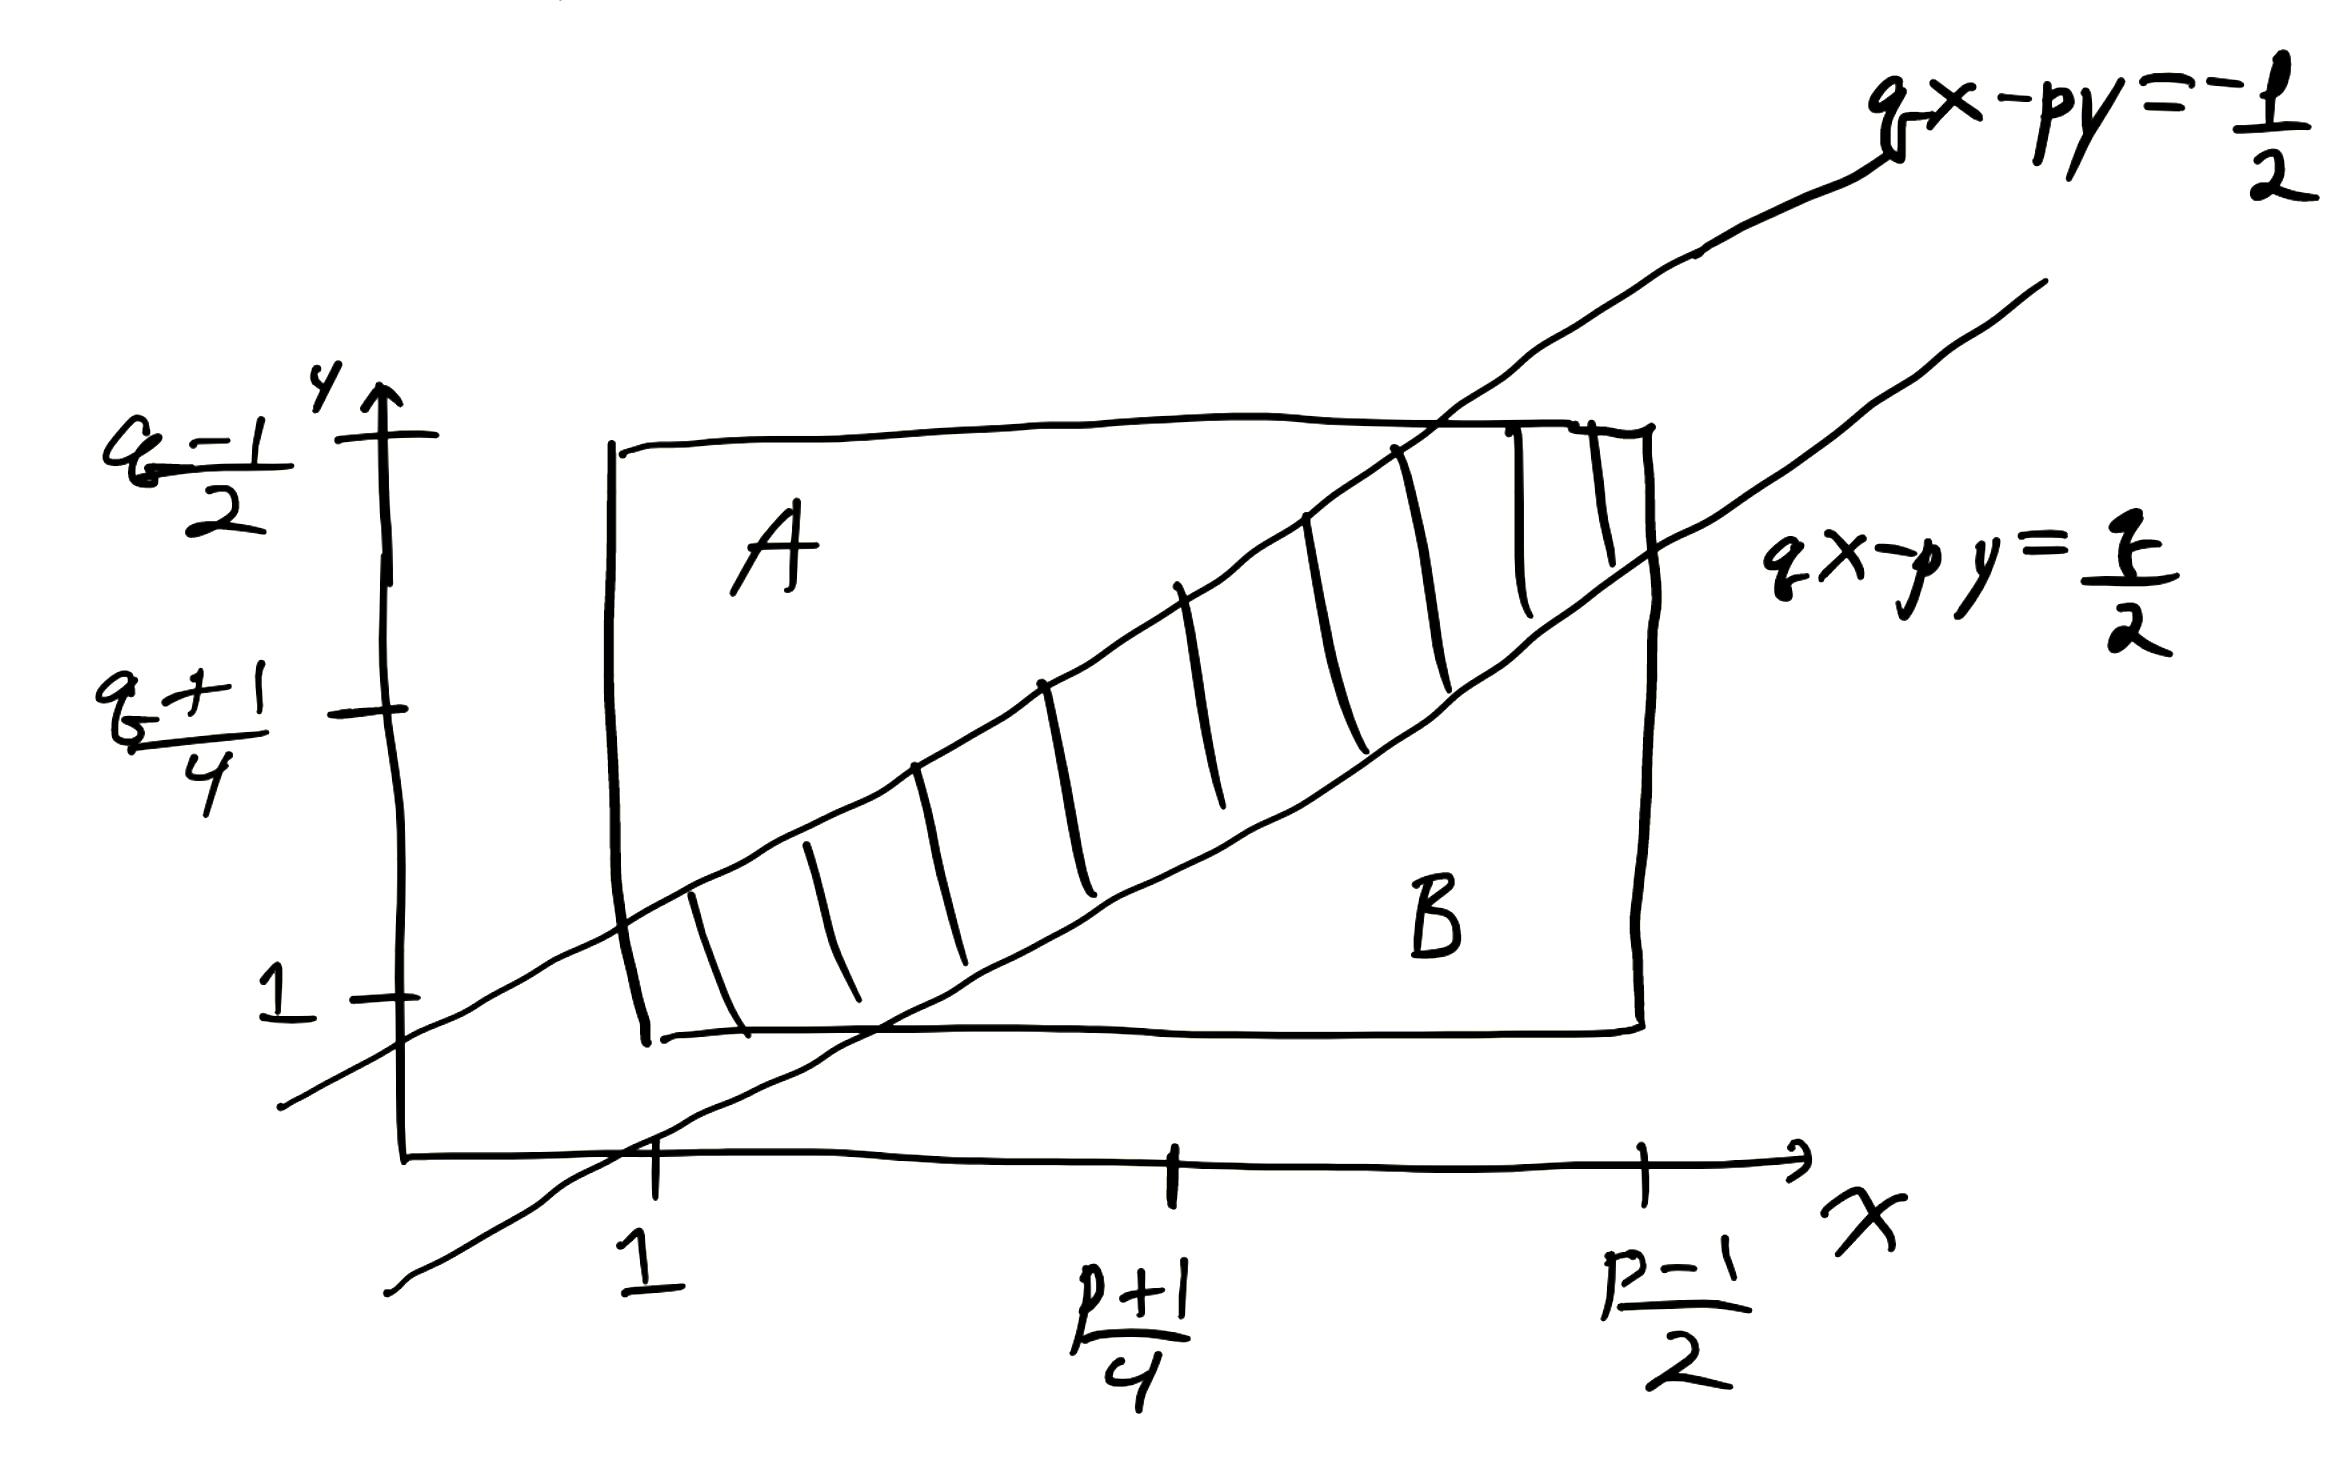
\includegraphics[width=0.8\textwidth]{images/qr-diagram.png}
    \end{center}

    where $\mu + \eta$ is the number of lattice points in the shaded region.

    If $\alpha$ is the number of lattice points in $A$ and $\beta$ the number of lattice points in $B$. Then
    \[\mu + \eta = \frac{p-1}{2}\frac{q-1}{2} - (\alpha + \beta)\]
    We show that $\alpha = \beta$ so that $\alpha + \beta \equiv 0\pmod{2}$.

    Let $\rho$ be the rotation given by rotating the rectangle about its center leaves it invariant.
    \[\rho(x, y) = \left(\frac{p+1}{2}-x, \frac{q+1}{2} - y\right)\]
    Quick check that
    \[qx - py < \frac{-p}{2} \Leftrightarrow qx' - py' > \frac{q}{2}\]

    Since $\rho$ maps lattice points to lattice points, then $\alpha = \beta$ which concludes the proof with a little extra handiwork.
\end{proof}

\subsection{Jacobi Symbol}
The Jacobi symbol generalizes the Legendre symbol.
\begin{definition}[Jacobi Symbol]
    Let $b$ be an odd positive integer and let $a\in\ZZ$. Write
    $b = p_1p_2\cdots p_m$, where $p_i$ are (not necessarily distinct) primes. Then we write
    \[\lege{a}{b} = \lege{a}{p_1}\lege{a}{p_2}\cdots \lege{a}{p_m}\]
    is called the \ul{Jacobi symbol}.
\end{definition}
We note some basic properties that the Jacobi symbol is totally multiplicative (on top and bottom!):
\begin{align*}
    \lege{a_1a_2}{b} & = \lege{a_1}{b}\lege{a_2}{b} \\
    \lege{a}{b_1b_2} & = \lege{a}{b_1}\lege{a}{b_2}
\end{align*}
\begin{remark*}
    Note that they're multiplicative \emph{fixing} either top or bottom. That is, they don't multiply like fractions.
\end{remark*}

\textbf{Warning!} $\lege{a}{b} = 1$ does not imply that $a$ is a quadratic residue modulo $b$ (since we could have $-1$'s from the factorization cancel out).

However, $\lege{a}{b} = -1$ \emph{does} imply that $a$ is a non-residue modulo $b$. (it is a non-residue mod at least one of prime factors of $b$).

\begin{example}
    \[\lege{2}{15} = \lege{2}{3}\lege{2}{5} = (-1)(-1) = 1\]
    but $2$ is not a quadratic residue modulo $15$.
\end{example}
\begin{proposition}[5.2.2 of Text]\label{prop:5.2.2}
    We have the following properties about the Jacobi symbol:
    \begin{enumerate}[(a)]
        \item \[\lege{-1}{b} = (-1)^{\frac{b-1}{2}}\]
        \item \[\lege{2}{b} = (-1)^{\frac{b^2 - 1}{8}}\]
        \item If $a, b\in\ZZ_+$, then
              \[\lege{a}{b}\lege{b}{a} = (-1)^{\frac{a-1}{2}\frac{b-1}{2}}\]
    \end{enumerate}
\end{proposition}
%!TEX root = ../notes.tex
\section{March 10, 2022}
\subsection{Jacobi Symbol \emph{continued}}
\recall
\begin{definition*}[Jacobi Symbol]
    Let $b\in\ZZ_+$ be odd, and let $a\in\ZZ$. We write $b = p-1p_2\cdots p_m$, where $p_i$ are primes (not necessarily distinct). Then we have
    \[\lege{a}{b} = \lege{a}{p_1}\lege{a}{p_2}\cdots \lege{a}{p_m}\]
    is called the \ul{Jacobi symbol}.
\end{definition*}

This generalizes the Legendre symbol. We have basic properties that
\begin{align*}
    \lege{a_1a_2}{b} & = \lege{a_1}{b}\lege{a_2}{b} \\
    \lege{a}{b_1b_2} & = \lege{a}{b_1}\lege{a}{b_2}
\end{align*}
We noted that $\lege{a}{b} = -1$ implies that $a$ is \emph{not} a quadratic residue mod $b$ but $\lege{a}{b} = 1$ does not imply $a$ is a quadratic residue mod $b$.

We also stated analogues of the reciprocity laws for the Legendre symbol.

\begin{lemma}\label{lemma:multiplicativity-for-jacobi}
    Let $r, s\in\ZZ_+$ be odd. Then
    \begin{enumerate}[(a)]
        \item $\displaystyle\frac{rs-1}{2}\equiv \frac{r-1}{2} + \frac{s-1}{2}\mod 2$.
        \item $\displaystyle\frac{r^2s^2 - 1}{8} \equiv \frac{r^2-1}{8} + \frac{s^2 - 1}{8}\mod 2$.
    \end{enumerate}
\end{lemma}
\begin{proof}
    ~\begin{enumerate}[(a)]
        \item $(r-1)(s-1)\equiv 0\mod 4$. Hence
              \begin{align*}
                  rs - 1 & \equiv (r-1)(s-1) + r + s - 2\mod 4          \\
                         & \equiv r + s - 2\mod{4}                      \\
                         & \equiv (r-1) + (s-1)\mod{4}                  \\
                         & \equiv \frac{r-1}{2} + \frac{s-1}{2} \mod{2}
              \end{align*}
              which gives (a).
        \item We follow the same procedure, more or less. $(r^2-1)(s^2-1)\equiv 0\mod{16}$, so
              \begin{align*}
                  r^2s^2-1 & \equiv (r^2-1)(s^2-1)+r^2+s^2-2\mod{16}         \\
                           & \equiv (r^2-1)+(s^2-1)\mod{16}                  \\
                           & \equiv \frac{r^2-1}{8} + \frac{s^2-1}{8}\mod{2}
              \end{align*}
              which gives (b).
    \end{enumerate}
\end{proof}

\begin{corollary}
    let $r_1, r_2, \dots, r_m\in\ZZ_+$ be odd. Then
    \begin{enumerate}[(a)]
        \item $\displaystyle
                  \sum_{i=1}^m \frac{r_i-1}{2} \equiv \frac{r_1r_2\cdots r_m - 1}{2}\mod 2
              $.
        \item $\displaystyle
                  \sum_{i=1}^m \frac{r_i^2 - 1}{2}\equiv \frac{r_1^2r_2^2\cdots r_m^2 - 1}{8}\mod 2
              $.
    \end{enumerate}
\end{corollary}
\begin{proof}
    By induction on $m$ from \cref{lemma:multiplicativity-for-jacobi}.
\end{proof}

We restate the reciprocity laws but for Jacobi symbols, \cref{prop:5.2.2}:
\begin{proposition*}[5.2.2 of Text]
    We have the following properties about the Jacobi symbol:
    \begin{enumerate}[(a)]
        \item \[\lege{-1}{b} = (-1)^{\frac{b-1}{2}}\]
        \item \[\lege{2}{b} = (-1)^{\frac{b^2 - 1}{8}}\]
        \item If $a, b\in\ZZ_+$, then
              \[\lege{a}{b}\lege{b}{a} = (-1)^{\frac{a-1}{2}\frac{b-1}{2}}\]
    \end{enumerate}
\end{proposition*}
\begin{proof}[Proof of \cref{prop:5.2.2}]
    ~\begin{enumerate}
        \item[(a) $+$ (b)] are immediate from the corollary (factor $b$, sum exponents and take the parity of the exponent) and the supplemental laws of quadratic reciprocity.
        \item[(c)] Let
            \begin{align*}
                a & =q_1q_2\cdots q_l   \\
                b & = p_1p_2\cdots p_m.
            \end{align*}
            Then
            \begin{align*}
                \lege{a}{b}\lege{b}{a} & = \prod_{i}\prod_{j} \lege{q_i}{p_j}\lege{p_i}{q_j}                                     \\
                                       & = (-1)^{\sum_i \sum_j \left(\frac{q_i-1}{2}\right)\left(\frac{p_j-1}{2}\right)}
                \intertext{Applying the corollary, }
                                       & = (-1)^{\left(\sum_i \frac{q_i - 1}{2}\right)\left(\sum_j \frac{p_j - 1}{2}\right)}     \\
                                       & = (-1)^{\left(\frac{(\sum_i q_i) - 1}{2}\right)\left(\frac{(\sum_j p_j) - 1}{2}\right)} \\
                                       & = (-1)^{\left(\frac{a-1}{2}\right)\left(\frac{b-1}{2}\right)}
            \end{align*}
            which is as desired!
    \end{enumerate}
\end{proof}
\begin{example}
    We try to compute with the Jacobi symbol. Recall \cref{example:legendre-symbol}
    \[\lege{219}{383}\]
    where we repeatedly factored and flipped. With a Jacobi symbol, we don't need to start with factoring; we can forego factorization of top argument and simply repeatedly flip:
    \begin{align*}
        \lege{219}{383} & = - \lege{383}{219} = -\lege{164}{219} = - \lege{4}{219}\lege{41}{219} = - \lege{41}{219} \\
                        & = - \lege{219}{41} = - \lege{14}{41} = - \lege{2}{41}\lege{7}{41} = -\lege{7}{41}         \\
                        & = -\lege{41}{7} = -\lege{-1}{7} = \boxed{1}.
    \end{align*}
\end{example}
What we did here is to exploit the fact that \emph{all} Legendre symbols agree with Jacobi symbols, we treat it as a Jacobi symbol and do `Jacobi-\emph{like}' manipulations on it.
\begin{center}
    
\includegraphics[width=0.4\textwidth]{images/jacobi_legendre_reveal.jpeg}
\end{center}

\emph{This marks the dividing line between the first half and latter half of the course! Everything up to this point is fair game on the midterm. We also now switch to Stewart and Tall.}

\subsection{Number Fields}
\begin{definition}[Algebraic Numbers]
    A complex number $x$ is called \ul{algebraic} if it is algebraic over $\QQ$, i.e., if it satisfies a nonzero polynomial equation over $\QQ$.

    We denote the set of algebraic numbers over $\QQ$ as $\overline{\QQ}$.
\end{definition}
\begin{proposition}
    The set $\overline{\QQ}$ of algebraic numbers is a subfield of $\CC$. That is, addition and multiplication is closed, and we have inverses for nonzero elements.
\end{proposition}
\begin{proof}
    The key point is that if $L / K$ is a field extension, then $\alpha\in L$ is algebraic over $K$ iff $K(\alpha)/K$ is finite.

    So suppose $\alpha, \beta\in\overline{\QQ}$. Then $\QQ(\alpha)/\QQ$ and $\QQ(\beta)/\QQ$ are finite. Thus $\QQ(\alpha, \beta)/\QQ$ is finite (and all pieces of the associated diamond are finite extensions as well).

    \[
        \xymatrix{
            \QQ \ar[d] \ar[r] &\QQ(\alpha)\ar[d]\\
            \QQ(\beta) \ar[r] &\QQ(\alpha, \beta)}
    \]


    Since $\alpha + \beta$, $\alpha - \beta$, $\alpha\beta$ and for $\beta \neq 0$, $\alpha/\beta \in \QQ(\alpha, \beta)$. This means that all of these elements are algebraic over $\QQ$.
\end{proof}

\begin{definition}
    A \ul{number field} is a subfield $K$ of $\CC$ such that $[K : \QQ] < \infty$.
\end{definition}

Thus every element of a number field is algebraic, so $K\subseteq \overline{Q}$.

By the definition of a finite extension, every number field has the form
\[K = \QQ(\alpha_1, \alpha_2, \dots, \alpha_N)\text{ for some }\alpha_1, \dots, \alpha_n\in\overline{\QQ}\]

However, something stronger than this holds.

\begin{theorem}[Primitive Element Theorem]
    If $K$ is a number field, then $K = \QQ(\theta)$ for some $\theta\in\overline{\QQ}$.
\end{theorem}
\begin{proof}[Proof sketch]
    It is enough to show that if
    \[K = K_1(\alpha, \beta), \]
    then $K = K_1(\theta)$ for some $\theta\in\overline{\QQ}$.

    Suppose the minimum polynomials (over $\QQ$) of $\alpha$ and $\beta$ respectively are (factored over roots in $\CC$):
    \begin{align*}
        (t-\alpha_1)(t-\alpha_2)\cdots (t-\alpha_n)\qquad \alpha_1 & = \alpha \\
        (t-\beta_1)(t-\beta_2)\cdots (t-\beta_n)\qquad \beta_1     & = \beta  \\
    \end{align*}
    These polynomials are separable. Hence for each $i$ and each $k\neq 1$, there exists at most one $x\in K_1$ such that
    \[\alpha_i + x\beta_k = \alpha_1 + x\beta_1.\]
    (This only holds for more $x$ when you have $\beta_k$ and $\beta_1$ colliding). There are only finitely many of these equations, so we can choose a nonzero $c\in K_1$ such that
    \[\alpha_i + c\beta_k \neq \alpha_1 + c\beta_1\]
    for any $1\leq i\leq n$ and $2\leq k\leq m$.

    Define $\theta = \alpha + c\beta$. We claim that
    \[K_1(\alpha, \beta) = K_1(\theta)\]
    for which the proof is on page 39 of Stewart Tall.
\end{proof}
%!TEX root = ../notes.tex
\section{March 15, 2022}
\subsection{Number Fields \emph{continued}}
\recall from last class...
\begin{definition*}
    A complex number $\alpha$ is called \ul{algebraic} if it is algebraic over $\QQ$.
\end{definition*}
\begin{proposition*}
    The set $\overline{\QQ}$ of algebraic numbers is a subfield of $\CC$.
\end{proposition*}
\begin{definition*}
    A number field is a subfield $K$ of $\CC$ such that $[K: \QQ]<\infty$.
\end{definition*}
\begin{theorem*}[Primitive Element Theorem]
    If $K$ is a number field, then $K = \QQ(\theta)$ for some $\theta\in \overline{\QQ}$.
\end{theorem*}
\begin{proof}[Crux of proof]
    Suppose $K = K_1(\alpha, \beta)$. Thus $K = K_1(\theta)$ for some $\theta$ that is easily found as a function of $\alpha$ and $\beta$.

    Write the minimum polynomials of $\alpha, \beta$ over $K_1$(factored over $\CC$)
    \begin{align*}
        (t-\alpha_1)(t-\alpha_2)\cdots (t-\alpha_n)\quad \alpha_i\in\overline{\QQ}, \text{ and }\alpha =: \alpha_1 \\
        (t-\beta_1)(t-\beta_2)\cdots (t-\beta_m)\quad \beta_i\in\overline{\QQ}, \text{ and }\beta =: \beta_1
    \end{align*}
    These are separable. Hence for each $i$ and each $k\neq 1$, there exists at most one $x\in K$ such that
    \[\alpha_i + x\beta_k = \alpha_1 + x\beta_1\]
    Hence, since there are only finitely many of these equations, we can choose $0\pm c\in K$, such that
    \[\alpha_i + c\beta_k \neq \alpha_1 + c\beta_1\]
    for any $1\leq i\leq n$ and $2\leq k\leq m$. We define $\theta = \alpha + c\beta$. We claim $K = K_1(\theta)$.
\end{proof}
The proof up to this claim is actually useful in finding a primitive element.
\begin{example}[p.39 \cite{stewart2015algebraic}]
    Let $K = \QQ(\sqrt{2}, \sqrt[3]{5})$.
    \[\alpha_1 = \sqrt{2}, \beta_1 = \sqrt[3]{5}\]
    We then have $\alpha_2 = -\sqrt{2}$ and we can let $\beta_2 = \zeta_3\sqrt[3]{5}, \beta_2 = \zeta_3^2\sqrt[3]{5}$ where $\zeta_3$ is the primitive 3rd root of unity.

    $c = 1$ has the property that
    \[\alpha_i + c\beta_k \neq \alpha_1 + c\beta_1\]
    for $1\leq i\leq 2$ and $2\leq k\leq 3$.

    Therefore, we can conclude that $\sqrt{2} + \sqrt[3]{5}$ is a primitive element for $\QQ(\sqrt{2}, \sqrt[3]{5})/\QQ$.
\end{example}

\subsection{Conjugates of Algebraic Numbers}
\begin{theorem}[p.40 \cite{stewart2015algebraic}]
    Let $K = \QQ(\theta)$ be a number field of degree $n$ over $\QQ$. Then there exists exactly $n$ distinct field embedding of $K$ into $\CC$. (We label these $\sigma_i : K \hookrightarrow \CC, 1\leq i \leq n$.)

    The $\sigma_i(\theta)=:\theta_i$ are the zeros in $\CC$ of the minimal polynomial of $\theta$ over $\QQ$.
\end{theorem}
\begin{proof}
    Suppose $\sigma : K\hookrightarrow \CC$ is an embedding. We have that $\sigma$ is the identity on $\QQ$ (since $\sigma(1) = 1$), so
    \[0=\sigma(f(\theta)) = f(\sigma(\theta))\qquad \text{where $f:= \minpoly_\QQ(\theta)$}.\]
    Hence $\sigma(\theta)$ is a root of $f$.

    Conversely, for each root $\theta_i$ of $f$, there is a field isomorphism\footnote{We find isomorphisms $\QQ(\theta)\overset{\sim}{\longrightarrow} \QQ[x]/f$ and similarly $\QQ(\theta_i)\overset{\sim}{\longrightarrow} \QQ[x]/f$ where $f :=\minpoly_\QQ(\theta) = \minpoly_\QQ(\theta_i)$.} taking
    \[\QQ(\theta)\overset{\sigma_i}{\longrightarrow}\QQ(\theta_i)\]
    such that $\sigma_i (\theta) = \theta_i$. Therefore we've shown a bijection between the roots of $f$ and the embeddings of $K$ into $\CC$.
\end{proof}

\subsection{Discriminants of Bases, Vandermonde Determinant}
Let $K = \QQ(\theta)$ be a number field of degree $n$, and let $\{\alpha_1, \alpha_2, \dots, \alpha_n\}$ be a basis of $K$ as a vector space over $\QQ$. Let $\sigma_i : K\hookrightarrow \CC$, $1\leq i\leq n$ be the embeddings of $K$ into $\CC$.

\begin{definition}
    The discriminant of $\{\alpha_1, \alpha_2, \dots, \alpha_n\}$ is
    \begin{align*}
        \Delta[\alpha_1, \alpha_2, \dots, \alpha_n] & = \det\left(\sigma_i(\alpha_i)\right)^2 \\
                                                    & = \det
        \begin{pmatrix}
            \sigma_1(\alpha_1) & \sigma_1(\alpha_2) & \cdots & \sigma_1(\alpha_n) \\
            \sigma_2(\alpha_1) & \sigma_2(\alpha_2) & \cdots & \sigma_2(\alpha_n) \\
            \vdots             & \vdots             & \ddots & \vdots             \\
            \sigma_n(\alpha_1) & \sigma_n(\alpha_2) & \cdots & \sigma_n(\alpha_n) \\
        \end{pmatrix}^2
    \end{align*}
\end{definition}
If $\{\beta_1, \dots, \beta_n\}$ is another basis, then $\forall 1\leq k\leq n$,
\[\beta_k = \sigma_{i = 1}^n C_{ik}\alpha_i, \quad C_{ik}\in \QQ,\]
where $\det(C_{ik})\neq 0$. Then it is a fact that
\[\Delta[\beta_1, \dots, \beta_n] = \left(\det(C_{ik})\right)^2\cdot \Delta[\alpha_1, \dots, \alpha_n]\]
\begin{theorem}[p.42 \cite{stewart2015algebraic}]\label{thm:2.7}
    The discriminant of any basis for $K = \QQ(\theta)$ is rational and nonzero.
\end{theorem}
\begin{proof}
    It suffices to show that this holds for $\{1, \theta, \theta^2, \dots, \theta^{n-1}\}$ by the above fact.

    Write $\theta = \theta_1$, $\theta_1, \theta_2, \dots, \theta_n$ for the conjugates of $\theta_1$. Then
    \[\Delta[1, \theta, \theta^2, \dots, \theta^{n-1}] = \left(\det(\theta_i^j)\right)^2\]
    We use a general observation
    \begin{definition}[Vandermonde Matrix]
        A (square) \ul{Vandermonde matrix} is a matrix of the form
        \[V = \begin{pmatrix}
                1      & t_1    & t_1^2  & \dots  & t_1^{n-1} \\
                1      & t_2    & t_2^2  & \dots  & t_2^{n-1} \\
                \vdots & \vdots & \vdots & \ddots & \vdots    \\
                1      & t_n    & t_n^2  & \dots  & t_n^{n-1} \\
            \end{pmatrix}\]
    \end{definition}
    \begin{claim}
        The determinant of $V$ is
        \[\prod_{1\leq i < j\leq n}(t_i - t_j).\]
    \end{claim}
    Going back to the proof of our claim about discriminants, we can take $t_i = \theta_i := \sigma_i(\theta)$ to get
    \begin{align*}
        \Delta[1, \theta, \dots, \theta^{n-1}] & = \prod_{i<j}(\theta_i - \theta_j)^2  \\
                                               & = \mathsf{disc}(\minpoly_\QQ(\theta))
    \end{align*}
\end{proof}
%!TEX root = ../notes.tex
\section{March 17, 2022}
\subsection{Midterm Review}
\subsubsection*{General Advice}
\begin{itemize}
    \item 5-7pm. Location: Barus \& Holley 168.
    \item There are 5 problems:
          \begin{itemize}
              \item Each are weighted equally, some have multiple sections in them.
              \item There is a bonus problem for a \emph{token} number of points.
          \end{itemize}
    \item Think about problems before starting! Don't begin immediately.
\end{itemize}

\subsubsection*{Key Topics}
\begin{enumerate}[1)]
    \item
          Unique factorization in $\ZZ$ (\cref{thm:unique-factorization}). Key points:
          \begin{itemize}
              \item Existence (using well-ordering of $\ZZ_+$)
              \item Uniqueness (using prime elements being irreducible elements in $\ZZ$)
          \end{itemize}
    \item
          $\ZZ$ is a Euclidean domain with Euclidean function $\mathsf{abs}$ (absolute value) (\cref{cor:z-euclidean}).
          \begin{itemize}
              \item Argument uses well-ordering of $\ZZ_+$ applied to the set $S = \{a - bq\mid b\in \ZZ\}$ when trying to divide $a$ by $b$.
              \item Repeated application of this property yields the Euclidean algorithm for finding $\gcd$'s.
          \end{itemize}
    \item
          Bezout's Identity (\emph{not} Bezout's Theorem)

          If $a, b\in\ZZ$ are integers (not both $0$) and $c\in \ZZ$, then there exists $x, y\in\ZZ$ such that
          \[ax + by = c\]
          if and only if $\gcd(a, b)\mid c$.
          \begin{itemize}
              \item We take set $S = \{ax + by\mid x, y\in\ZZ\}$ and use well-ordering to show that the smallest element has to be $c$.
          \end{itemize}
    \item
          From Bezout to solving linear congruences in $1$ variable, the linear congruence
          \[ax\equiv b\pmod{m}\]
          is equivalent to
          \[ax - my = b\]
          for some $y\in \ZZ$. Applying Bezout's tells us that this equation is solvable if and only if $\gcd(a, b)\mid b$. When a solution exists, there are $d$ solutions modulo $m$.
          \begin{itemize}
              \item Showing there are $d$ solutions: you divide $a, b, m$ by $\gcd(a, m)$, then you have a modulus $\frac{m}{\gcd(a, m)}$ where we have a unique solution. We lift up to solutions modulo $m$.
          \end{itemize}
    \item
          Sunzi's theorem (\cref{thm:crt}). For $m, n\in\ZZ_+$ with $(m, n) = 1$. And $a, b\in\ZZ$, then the simultaneous congruences
          \begin{align*}
              x\equiv a\pmod{m} \\
              x\equiv b\pmod{n}
          \end{align*}
          have a \emph{unique} solution modulo $mn$.
          \begin{itemize}
              \item We have $\pi : \ZZ/mn\ZZ\to \ZZ/m\ZZ\times \ZZ/n\ZZ$ be the natural projectsion where $\ker(\pi) = \{0\}$ since $(m, n) = 1$.
          \end{itemize}
    \item
          Structure of group of units (\cref{cor:cyclicity-of-unit-groups}). $U(m)$ is cyclic $\iff$ $m = 1, 2, 4, p^e, 2p^e$.
\end{enumerate}

\subsubsection*{Practice Problems}
\begin{problem}
Find the integer $0\leq a\leq 36$ such that
\[3777^{\left(1144523^{56245501}\right)} \equiv a\pmod{37}\]
\end{problem}
We can reduce the base $3777\equiv 3\pmod{37}$. We reduce $1144523\equiv 11\pmod{\phi(37)}$. We can reduce the upper power $56245501\equiv 1\pmod{\phi(\phi(37))}$. This reduces to
\[3^{11}\equiv a\pmod{37}\]
which gives $a\equiv 28\pmod{37}$.

\begin{problem}
Let $p\in\ZZ$ be a prime and let $g$ be a primitive root mod $p$. Describe the set
\[\{g^k\mid g^k \text{ is a primitive root mod $p$}\}\]
\end{problem}
\begin{proof}
    We claim that $\gcd(k, p-1) = 1$. Then for any element $a = g^\alpha$, we can find power $(g^k)^\beta = g^\alpha$ since we have $g^{p-1}\equiv 1$ so $k\beta - x(p-1) = \alpha$ for some $x$, which only has solutions by Bezout's identity when $\gcd(k, p-1)$.
\end{proof}

\begin{lemma*}
    Prove that for any finite group $G$ of order $n$ and any $g\in G$, the cyclic group $\langle g^k\rangle$ for $k$ such that $\gcd(k, \ord(g)) = 1$ equals $\langle g\rangle$.
\end{lemma*}
\begin{proof}
    Let $d = (k, \ord(g))$. Then there exists $x, y\in\ZZ$ such that
    \[\ord(g)\cdot x + k\cdot y = d\]
    so
    \begin{align*}
        g^d & = g^{\ord(g)\cdot x + ky}        \\
            & = g^{\ord(g)\cdot x}\cdot g^{ky} \\
            & = g^{ky}
    \end{align*}
    so $g^d\in \langle g^k\rangle \implies \langle g^d\rangle \subseteq \langle g^k\rangle$. We have $\langle g^k\rangle\subseteq \langle g^d\rangle$ since $d\mid k$. Thus $\langle g^d\rangle = \langle g^k\rangle$.

    We also have that $(g^k)^{\ord(g)/d} = (g^{\ord{g}})^{k/d} = 1$ so if $d = (k, \ord(g))>1$ then $\ord(g^k)< \ord(g)$.

    So together we have that $\langle g\rangle = \langle g^k\rangle$ if and only if $(g, \ord(g))=1$.
\end{proof}

\begin{problem}
Prove
\begin{proposition*}
    If $f : \ZZ_+\to \CC$ is a nonzero multiplicative function, then $f^{-1}$ (the Dirichlet inverse) exists and is multiplicative.
\end{proposition*}
\end{problem}
\begin{proof}
    Let $h$ be given by
    \begin{align*}
        h(p^k) & = f^{-1}(p^k)\qquad\text{prime powers $p^k$} \\
        h(n)   & = h(p_1^{e_1})\cdots h(p_k^{e_k})
    \end{align*}
    then $(f\star h)(p^k) = I(p^k)$. Both $f\star h$ and $I$ are multiplicative, so
    \[(f\star h)(n) = I(n)\quad\forall n\in\ZZ\]
    and $h = f^{-1}$.

    (Existence, $f(1) = 1$ for any multiplicative function, so in particular our given $f$ satisfies $f(1)\neq 0$.)
\end{proof}

\begin{problem}
Define $\lambda : \ZZ_+\to \CC$ by
\[\lambda(n) = (-1)^{e_1 + e_2 + \cdots}\]
where the $e_i$'s are the exponents on the prime factorization of $n$. Let
\[g(n) = \sum_{d\mid n}\lambda(d)\]
Prove that
\[g(n) = \begin{cases}
        1 & \text{if $n$ is square} \\
        0 & \text{otherwise}
    \end{cases}\]
\end{problem}
\begin{proof}
    We note that $\lambda$ is multiplicative, and $g$ is a summatory function of $\lambda$ which is multiplicative. So we just prove on prime powers. If we have prime power with even exponent, then $p, p^2, \dots, p^{e_1}\mid p^{e_1}$ gives $1 + (-1) + 1 + (-1) + \cdots + 1 = 1$. We have $0$ otherwise.
\end{proof}
%!TEX root = ../notes.tex
\section{March 22, 2022}
\subsection{Discriminants of bases, Vandermonde determinants}
We have some review from last time:

Let $K = \QQ(\theta)$ be a number field of degree $n$, let $\{\alpha_1, \dots, \alpha_n\}$ be a $\QQ$-basis of $K$, and let $\sigma_i : K\hookrightarrow \CC$, $1\leq i\leq n$ be the embeddings of $K$ into $\CC$.

The discriminant of $\{\alpha, \dots, \alpha_n\}$ is
\[\Delta[\alpha_i, \dots, \alpha_n] = \det\begin{pmatrix}
        \sigma_1(\alpha_1) & \sigma_1(\alpha_2) & \cdots & \sigma_1(\alpha_n) \\
        \sigma_2(\alpha_1) & \sigma_2(\alpha_2) & \cdots & \sigma_2(\alpha_n) \\
        \vdots             & \vdots             & \ddots & \vdots             \\
        \sigma_n(\alpha_1) & \sigma_n(\alpha_2) & \cdots & \sigma_n(\alpha_n) \\
    \end{pmatrix}^2\]

If $\{\beta_1, \dots, \beta_n\}$ is another basis, then for all $1\leq k\leq n$,
\[\beta_k = \sum_{i=1}^n c_{ik}\alpha_i, \quad c_{ik}\in \QQ,\]
where $\det(c_{ik})\neq 0$. Fact from homework is that
\[\Delta[\beta_i, \dots, \beta_n] = \det(c_{ik})^2\cdot \Delta[\alpha_i, \dots, \alpha_n]\]

\begin{theorem*}[2.7, p.42 \cite{stewart2015algebraic}]
    The discriminant of any $\QQ$-basis for $K$ is rational and nonzero.
\end{theorem*}
\begin{proof}
    It suffices to prove this for $\{1, \theta, \theta^2, \dots, \theta^{n-1}\}$.
\end{proof}

We have the following observation:
\begin{definition*}[Vandermonde Matrix]
    A (square) \ul{Vandermonde matrix} is a matrix of the form
    \[V = \begin{pmatrix}
            1      & t_1    & t_1^2  & \dots  & t_1^{n-1} \\
            1      & t_2    & t_2^2  & \dots  & t_2^{n-1} \\
            \vdots & \vdots & \vdots & \ddots & \vdots    \\
            1      & t_n    & t_n^2  & \dots  & t_n^{n-1} \\
        \end{pmatrix}\]
\end{definition*}

We then claimed (without proof) that
\begin{claim*}
    The determinant of $V$ is
    \[\prod_{1\leq i < j\leq n}(t_j - t_i).\]
\end{claim*}
\begin{proof}
    We know that $\det(V) = 0$ when $t_i = t_j$ for some $i\neq j$. So, $\det(V)$ (as a polynomial in $t_1, \dots, t_n$) is divisible by $t_i - t_j$ for $i < j$. We have that the total degree of $\det(V)$ as a polynomial in $t_1, \dots, t_n$ is
    \[\sum_{i=1}^{n-1} i = \frac{n(n-1)}{2}.\]
    On the other hand, the total degree of $D$ is also $\binom{n}{2} = \frac{n(n-1)}{2}$. Hence, $\det(V)$ is a scalar multiple of $D$ (since ).

    But $\det(V)$ and $D$ are both monic as polynomials (\emph{kinda}) in $\QQ(t_2, \dots, t_n)[t_1]$. Thus $\det(V) = D$. \emph{Or something like that}.
\end{proof}

Going back to the proof of \cref{thm:2.7}, we take $t_i = \theta_i := \sigma_i(\theta)$ to get
\begin{align*}
    \Delta[1, \theta, \dots, \theta^{n-1}] & = \prod_{i < j}(theta_i - \theta_j)^2  \\
                                           & = \mathsf{disc}(\minpoly_\QQ(\theta)).
\end{align*}
which is clearly rational and nonzero in $\QQ^+$.

\begin{example}
    Let
    \[K = \QQ(\sqrt{5})\]
    with the obvious basis $\{1, \sqrt{5}\}$. We have
    \begin{align*}
        \Delta[1, \sqrt{5}] & = \left|\begin{array}{cc}
                                          1 & \sqrt{5}  \\
                                          1 & -\sqrt{5}
                                      \end{array}\right|^2 \\
                            & = (-2\sqrt{5})^2             \\
                            & = 20
    \end{align*}
    and another basis is $\left\{1, \frac{1+\sqrt{5}}{2}\right\}$ and
    \begin{align*}
        \Delta\left[1, \frac{1+\sqrt{5}}{2}\right] & = \left|\begin{array}{cc}
                                                                 1 & \frac{1+\sqrt{5}}{2}  \\
                                                                 1 & -\frac{1+\sqrt{5}}{2}
                                                             \end{array}\right|^2 \\
                                                   & = (-2\frac{\sqrt{5}}{2})^2                      \\
                                                   & = (\sqrt{5})^2 = 5
    \end{align*}
\end{example}

\begin{example}
    Let
    \[K = \QQ(\sqrt[3]{2})\]
    A basis is $\{1, \sqrt[3]{2}, (\sqrt[3]{2})^2\} =: B$
    \begin{align*}
        \Delta(B) = \left|\begin{array}{ccc}
                              1 & \sqrt[3]{2}          & (\sqrt[3]{2})^2          \\
                              1 & \zeta_3\sqrt[3]{2}   & (\zeta_3\sqrt[3]{2})^2   \\
                              1 & \zeta_3^2\sqrt[3]{2} & (\zeta_3^2\sqrt[3]{2})^2
                          \end{array}\right|
    \end{align*}
    \emph{computation left as exercise\dots}
\end{example}

\subsection{Algebraic Integers}
\begin{definition}[Algebraic Integer]
    A complex number is an \ul{algebraic integer} if it is a root of a \emph{monic} polynomial with integer coefficients.
\end{definition}

We denote the set of algebraic integers by $\overline{\ZZ}$. By definitions, $\overline{\ZZ}\subseteq\overline{\QQ}$.

\begin{example}
    The following are some algebraic integers: 
    \begin{itemize}
        \item $\sqrt{2}\in\overline{\ZZ}$ since $\sqrt{2}$ is a root of $x^2 - 2$. 
        \item $\tau = \frac{1}{2}(1 + \sqrt{5})$, since $\tau^2 - \tau - 1 = 0$. 
    \end{itemize}
    Non-examples: 
    \begin{itemize}
        \item $\frac{22}{7}$ is not an algebraic integer. \emph{Why?} We look at the $7$-adic valuation of the monic polynomial when we plug $\frac{22}{7}$ in. What are some other ways to reason about this? 
    \end{itemize}
\end{example}
Key algebra fact: If $f(x)\in \ZZ[x]$ is a monic polynomial with $f(x) = g(x)\cdot h(x)$ where $g(x)$, $h(x)$ are monic polynomials in $\QQ[x]$, then $g(x), h(x)\in \ZZ[x]$. (Gauss's Lemma). 

Hence, if $\frac{22}{7}$ is an algebraic integer, if has some $f(x)\in\ZZ[x]$ for which it is a root. But it is also a root of $g(x) = x - \frac{22}{7}$ where $f(x) = g(x)\cdot h(x)$ forcing $g(x)$ to be in $\ZZ[x]$. So the fact that $\minpoly_\QQ\left(\frac{22}{7}\right) = x - \frac{22}{7}$ implies that $\frac{22}{7}\not\in\overline{\ZZ}$. 

\begin{definition*}[Algebraic Integer']
    An algebraic number $\theta$ is an algebraic integer iff $\minpoly_\QQ(\theta)\in\ZZ[x]$. 
\end{definition*}
%!TEX root = ../notes.tex
\section{March 24, 2022}
\subsection{Algebraic Integers \emph{continued}}
\recall our definition for algebraic integers\dots
\begin{definition*}[Algebraic Integer]
    A complex number that satisfies $f(x) = 0$ for a non-constant \emph{monic} polynomial $f(x)\in\ZZ[x]$ is an \ul{algebraic integer}.

    An algebraic number is an algebraic number whose minimal polynomial over $\QQ$ has integer coefficients.

    We denote this set by $\ZZbar$.
\end{definition*}

Clearly, we have that $\ZZbar \subseteq \QQbar$.
\begin{claim*}
    We want to show that $\ZZbar$ is, in fact, a subring of $\QQbar$.
\end{claim*}

\begin{lemma}[Setup Lemma, p.44 \cite{stewart2015algebraic}]
    $\theta\in\CC$ is an algebraic integer iff the additive group generated by all powers $1, \theta, \theta^2, \dots$, $\ZZ[\theta, \theta^2, \dots]$, is finitely generated.
\end{lemma}
\begin{proof}
    \begin{description}
        \item[Forward Direction.] Suppose $\theta\in\ZZbar$. Then for some $n$,
            \[\theta^n  + a_{n-1}\theta^{n-1} + \cdots + a_0 = 0,\]
            where $a_i\in\ZZ, \forall\ 0\leq i\leq n-1$.
            \begin{claim*}
                Every power of $\theta$ lies in the additive group $\Gamma$ generated by $1, \theta, \theta^2, \dots, \theta^{n-1}$.
            \end{claim*}
            Suppose inductively that $m\geq n$, and that $1, \theta, \theta^2, \dots, \theta^m\in\Gamma$. We express
            \begin{align*}
                \theta^{n+1} = \theta^{m+1-n}\theta^n & = \theta^{m+1-n}(-a_{n-1}\theta^{n-1} - \cdots - a_0)     \\
                                                      & = -a_{n-1}\theta^m - \text{lower degree stuff} \in \Gamma
            \end{align*}
        \item[Backward Direction.] Suppose every power of $\theta$ lies in a finitely generated additive group $G$. Then the subgroup $\Gamma$ of $G$ generated by $\left\{ 1, \theta, \theta^2, \dots \right\}$ must also be finitely generated.

            Let $v_1, \dots, v_n$ be generators of $\Gamma$. (\textsc{wlog} can assume not all zero). Each $v_i \in\ZZ[\theta]$ (polynomial in $\theta$ with integer coefficients), so $\theta v_i\in\ZZ[\theta]\ \forall i$. Hence there exists integers $b_{ij}$ such that
            \[\theta v_i = \sum_{j=1}^n b_{ij}v_j\quad \forall i.\]
            This gives us a system of linear equations
            \begin{align*}
                (b_{11}-\theta)v_1 + b_{12}v_2 + \cdots + b_{1n}v_n & = 0    \\
                b_{21}v_1 + (b_{22}-\theta)v_2 + \cdots + b_{2n}v_n & = 0    \\
                                                                    & \vdots \\
                b_{n1}v_1 + b_{n2}v_2 + \cdots + (b_{nn}-\theta)v_n & = 0
            \end{align*}
            So now we have $A\vec{v} = \vec{0}$ so $\det{A} = 0$.

            The $v_1, \dots, v_n\in \CC$ give a nontrivial solution to the obvious associated system of linear equations, so the determinant
            \[\left|\begin{array}{cccc}
                    b_{11} - \theta & b_{12}          & \cdots & b_{1n}          \\
                    b_{21}          & b_{22} - \theta & \cdots & b_{2n}          \\
                    \vdots          & \vdots          & \ddots & \vdots          \\
                    b_{n1}          & b_{n2}          & \cdots & b_{nn} - \theta
                \end{array}\right|\]
            is zero. So the determinant, expanding as minors as a polynomial, is a monic\footnote{The highest degree of $\theta$ comes from the diagonal which monic up to sign. We also have that this is the characteristic of the $b_{ij}$ matrix which is monic.} polynomial (in $\theta$) with integral entries $b_{ij}$ of which $\theta$ satisfies. So $\theta$ is an algebraic integer.
    \end{description}
    Both directions of which are as desired.
\end{proof}

Note we prove something stronger and more intuitive:
\begin{lemma*}
    $\theta\in\CC$ is an algebraic integer iff the additive subgroup generated by $1, \theta, \theta^2, \dots$ is in fact generated by $1, \theta, \theta^2, \dots, \theta^{n-1}$ for some $n$.
\end{lemma*}
\begin{theorem}
    $\ZZbar$ is a subring of $\QQbar$.
\end{theorem}
\begin{proof}
    Suppose that $\theta, \phi\in\ZZbar$. We want to show that $\theta + \phi, \theta\phi\in\ZZbar$.

    By the lemma, all powers of $\theta$ lie in a finitely generated subgroup $\Gamma_\theta$ of $\CC$ and similarly, all powers of $\phi$ lie in a finitely generated subgroup $\Gamma_\phi$ of $\CC$.

    \otoh, all powers of $\theta + \phi$ and $\theta\phi$ are integer linear combinations of the elements
    \[\theta^k \phi^l\in \Gamma_\theta\Gamma_\phi\]
    where $\Gamma_\theta\Gamma_\phi := $ the additive group generated by $v_iw_j$ where $1\leq i\leq n$ and $1\leq j\leq m$ with
    \begin{align*}
        \Gamma_\theta & = \langle v_1, \dots, v_n\rangle \\
        \Gamma_\phi   & = \langle w_1, \dots, w_m\rangle
    \end{align*}
    We note that $\Gamma_\theta\Gamma_\phi$ is finitely generated, and since each power of $\theta+\phi$ and $\theta\phi$ lie in this finitely generated subgroup\footnote{The subgroup that they generate had better be finitely generated.}, by our lemma $\theta + \phi$ and $\theta\phi$ are both algebraic integers.
\end{proof}

\begin{theorem}[p.44 or p.45 \cite{stewart2015algebraic}]
    Let $\theta\in\CC$ satisfy a monic polynomial equation with coefficients in $\ZZbar$ (not just in $\ZZ$). Then $\theta$ is an algebraic integer.
\end{theorem}
\begin{proof}
    \emph{One imitates the proof of the forward direction in our previous setup lemma, applying a bit of module theory.}
\end{proof}

\subsection{Ring of Integers of a Number Field}
\begin{definition}[Ring of Integers of Number Field $K$]
    If $K$ is a number field, then
    \[\riO_K := K\cap \ZZbar\]
    is called the \ul{ring of integers of $K$}.\footnote{In textbooks, it's \emph{fraktor} $\riO$. In papers, usually mathcal $\mathcal{O}$. In handwriting, usually fancy loopy $O$.}
\end{definition}
$\riO_K$ is a ring because $K$ and $\ZZbar$ are subrings of $\CC$. The relationship between $K$ and $\riO_K$ is the same as that of $\QQ$ and $\ZZ$.

\begin{lemma}
    If $\alpha\in K$, then $c\alpha\in \riO_K$ for some $c\in\ZZ$.
\end{lemma}
\begin{proof}
    Let $\alpha\in K$ and $f(x) = \minpoly_\QQ(\alpha)$, with $\deg f = n$. Let $0\neq c\in \ZZ$ and let $g_c := c^n\cdot f\left( \frac{x}{c} \right)$.

    Observe:
    \begin{enumerate}[1)]
        \item The roots of $g_c$ are the $c\alpha_i$ where $\alpha_i$ are the roots of $f$.
        \item $g_c$ is monic.
        \item If we choose $c$ to be the lcm of the denominators of the coefficients of $f$ implies that $g_c$ has integer coefficients.
    \end{enumerate}
    So $c\alpha$ is an element of $\riO_K$ since it is also an algebraic integer.
\end{proof}

\begin{corollary}
    If $K$ is a number field, then $K = \QQ(\theta)$, for some algebraic integer $\theta\in\ZZbar$.
\end{corollary}

\textbf{Warning!} (pp.46-47 \cite{stewart2015algebraic}) Though it is often the case that if $K = \QQ(\theta)$ with $\theta\in\ZZbar$, then $\riO_K = \ZZ[\theta]$, this need not be true.
\begin{example}
    Let $K = \QQ(\sqrt{5})$. However,
    \[\ZZ[\sqrt{5}]\subsetneq \riO_K\]
    In fact, \[\ZZ\left[ \frac{1+\sqrt{5}}{2} \right] = \riO_K.\]
\end{example}
Furthermore, is it always the case that $\riO_K$ is generated by a single element? \emph{No!} $\riO_K$ need \ul{not} be of the form $\ZZ[\theta]$ for some $\theta\in\ZZbar$.
\begin{example}
    The counterexample of this is
    \[K = \QQ(\theta)\]
    when $\theta$ is a root of $x^3 - x^2 - 2x - 8$.
\end{example}
Number fields where such a $\theta$ does exist are called \ul{monogenic}.
%!TEX root = ../notes.tex
\section{April 5, 2022}
\subsection{Integral Bases for Number Fields}
\recall
\begin{itemize}
    \item We introduced embeddings of a number field $K$ into $\CC$, which was directly related to the notion of conjugates.
    \item Also introduced discriminants of $\QQ$-bases of number fields.
    \item Also introduced algebraic integers (algebraic numbers whose minimal polynomials over $\QQ$ have integral coefficients).
    \item We said that the \ul{ring of integers} of $K$ is by definition $\riO_K = K\cap \ZZbar$.
          \begin{itemize}
              \item If $K = \QQ$, then $\riO_K = \ZZ$.
          \end{itemize}
\end{itemize}

\begin{definition}[Integral Basis]
    Suppose $\mathcal{B} = \left\{ \alpha_1, \dots, \alpha_n \right\}$ is a $\QQ$-basis for $K$ such that $\alpha_i\in \riO_K\ \forall i$. We say that $\mathcal{B}$ is an \ul{integral basis} for $\riO_K$ if every element $\alpha\in\riO_K$ can be expressed \emph{uniquely} as
    \[\alpha = a_1\alpha_1 + a_2\alpha_2 + \cdots + a_n\alpha_n\]
    where each $a_i\in\ZZ$.
\end{definition}
\begin{theorem}
    Every number field has an integral basis.
\end{theorem}
\begin{example}
    Sometimes, we're lucky or it's obvious. For example, if $K = \QQ(\sqrt{2})$ then the obvious basis $\mathcal{B} = \{1, \sqrt{2}\}$ is an integral basis.
\end{example}
\begin{proof}
    Let $K$ be a number field of degree $n$. We had noted that if $\left\{ \alpha_1, \dots, \alpha_n \right\}$ is a $\QQ$-basis of $K$ with $\alpha_i\in \riO_K\ \forall i$, then
    \[\Delta\left[ \alpha_1, \alpha_2, \dots, \alpha_n \right]\in\ZZ\]
    We take the absolute value and apply a well-ordering argument. Let $\{\omega_1, \dots, \omega_n\}$ be a $\QQ$-basis with $\omega_i\in\riO_K\ \forall i$ and
    \[|\Delta\left[ \omega_1, \dots, \omega_n \right]|\leq |\Delta\left[ \alpha_1, \dots, \alpha_n \right]|\]
    for any $\QQ$-basis $\left\{ \alpha_1, \dots, \alpha_n \right\}$ with $\alpha_i\in \riO_K\ \forall i$ (it has the least absolute value of discriminant).

    \begin{claim*}
        $\{\omega_1, \dots, \omega_n\}$ is an integral basis for $\riO_K$.
    \end{claim*}
    Suppose otherwise, that there is an $\omega\in\riO_K$ such that $\omega = a_1\omega_1 + a_2\omega_2 + \dots + a_n\omega_n$ where $\alpha_i\in\QQ$ and at least one $a_i\not\in\ZZ$.

    \textsc{wlog} suppose $a_1\not\in\ZZ$. Then we can write
    \[a_1 = a + r\]
    where $a$ is an integer and $0\leq r\leq 1$.

    Let
    \begin{align*}
        \psi_1 & = \omega - a\omega_1 \\
        \psi_i & = \omega_i
    \end{align*}
    for the remaining indices. We check that these are integers $\psi_i\in\riO_K\ \forall i$ which is immediate since $\riO_K$ is a ring.

    The matrix sending the $\omega_i$'s to the $\psi_i$ (with respect to the $\omega_i$-basis) is
    \[M = \begin{pmatrix}
            a_1 - a & 0      & 0      & \cdots & 0      \\
            a_2     & 1      & 0      & \cdots & 0      \\
            a_3     & 0      & 1      & \cdots & 0      \\
            \vdots  & \vdots & \vdots & \ddots & \vdots \\
            a_n     & 0      & 0      & \cdots & 0
        \end{pmatrix}\]
    Since this matrix is lower triangular, the determinant is the product of the diagonal entries, namely: $a_1 - a = r$.\footnote{A nonzero determinant gives that $M$ is indeed a \emph{change-of-basis} matrix. So this is indeed a basis.}

    Hence,
    \begin{align*}
        \Delta[\psi_1, \psi_2, \dots, \psi_n] & = (\det M)^2\Delta[\omega_1, \omega_2, \dots, \omega_n] \\
                                              & = r^2\Delta[\omega_1, \omega_2, \dots, \omega_n]
    \end{align*}
    contradicting the minimality of $\left\{ \omega_1, \dots, \omega_n \right\}$ with respect to $|\Delta|$.

    Thus $\left\{ \omega_1, \dots, \omega_n \right\}$ is an integral basis for $K$.
\end{proof}
\begin{remark}
    A bit of extra reflection shows that \ul{any} integral basis has a discriminant achieving this minimal possible absolute value.
\end{remark}

\begin{ques*}
    How do you know if you're looking at an integral basis?
\end{ques*}
You can \emph{sometimes} diagnose this from the discriminant.
\begin{theorem}[p.50 \cite{stewart2015algebraic}]
    Suppose $\left\{ \alpha_1, \dots, \alpha_n \right\}$, with $\alpha_i\in\riO_K\ \forall i$ forms a $\QQ$-basis for $K$. If $\delta[\alpha_1, \dots, \alpha_n]$ is squarefree, then $\{\alpha_1, \dots, \alpha_n\}$ is an integral basis.
\end{theorem}
\begin{proof}
    Let $\{\beta_1, \beta_2, \dots, \beta_n\}$ is an integral basis. Then $\exists c_{ij}\in\ZZ$ such that each
    \[\alpha_i = \sum_{j}c_{ij}\beta_j\ \forall i.\]
    Then $M= (c_{ij})$ is the change of basis matrix from the $\alpha_i$'s to the $\beta_i$'s.
    \[\Delta[\alpha_1, \dots, \alpha_n] = (\det M)^2 \Delta[\beta_1, \dots, \beta_n]\]
    We know both $\det M$ and $\Delta[\beta_1, \dots, \beta_n]$ are integers and $\Delta[\alpha_1, \dots, \alpha_n]$ is squarefree. This forces $\det M = \pm 1$ so in fact $\{\alpha_1, \dots, \alpha_n\}$ is an integral basis.
\end{proof}
\begin{example}
    Let $K = \QQ(\sqrt{5})$. We previously observed that $\theta = \frac{1+\sqrt{5}}{2}\in\ZZbar$ hence $\theta\in\riO_K$ ($\theta$ is a root of $x^2 - x - 1$).
    \[\Delta\left[ 1, \frac{1+\sqrt{5}}{2} \right] = \left|\begin{array}{cc}
            1 & \frac{1+\sqrt{5}}{2} \\
            1 & \frac{1-\sqrt{5}}{2}
        \end{array}\right| = (-\sqrt{5})^2 = 5\]
    thus $\left\{ 1, \frac{1+\sqrt{5}}{2} \right\}$ is an integral basis for $K$.
\end{example}

We previously said that the discriminant of integral bases are invariant for each number field, so we give this a name:
\begin{definition}[Discriminant of Number Field]
    Let $K$ be a number field. The discriminant associated to any integral basis of $\riO_K$ is called the \ul{discriminant} of $K$.
\end{definition}
\begin{example}
    The discriminant of $K = \QQ(\sqrt{5})$ has $\disc(K) = 5$ (by previous computation).
\end{example}
\begin{example}
    What about $K = \QQ(\sqrt{2})$, $\riO_K = \ZZ[\sqrt{2}]$? We have
    \[\left|\begin{array}{cc}1 & \sqrt{2} \\ 1 & -\sqrt{2}\end{array}\right|^2 = (-2\sqrt{2})^2 = 8\]
    What if we don't want to do linear algebra? Previously we had that with power bases and Vandermonde discriminants, the discriminant of the basis is the discriminant of the minimum polynomial. $\{1, \sqrt{2}\}$ yields minimum polynomial $x^2 - 2$ which has determinant $8$.
\end{example}
\begin{example}
    More interesting, $K = \QQ(\theta)$ for $\theta$ a root of
    \[x^3 - x^2 - 2x - 8\]
    An integral basis for $\riO_K$ is given by
    \[\left\{ 1, \theta, \frac{\theta + \theta^2}{2} \right\}\]
    which is a number field that doesn't have a power integral basis. We have no basis of form $\{1, \omega, \omega^2, \dots, \omega^{n-1}\}$. The discriminant of this number field is $-503$.
\end{example}
Note: the following are ``synonyms'':
\begin{enumerate}
    \item $\riO_K = \ZZ[\theta]$ for some $\theta\in\ZZbar$, $\theta\in\riO_K$.
    \item $\riO_K$ (or $K$) is \ul{monogenic}.
    \item $\{1, \theta, \theta^2, \dots, \theta^{n-1}\}$ with $\deg\theta = n$ forms an integral basis for some $\theta\in\riO_K$.
    \item $\riO_K$ (or $K$) has a \ul{power integral basis}.
\end{enumerate}

We'll look at in more detail quadratic fields and cyclotomic extensions.

\subsection{Quadratic Fields}
\begin{definition}[Quadratic Field]
    A \ul{quadratic field} is a number field of degree $2$ over $\QQ$. For $K$ to be quadratic is for $K = \QQ(\theta)$ where $\theta$ a root of $x^2 + ax + b$, $a, b\in\ZZ$.
\end{definition}
This gives that $\theta = \frac{-a \pm \sqrt{a^2 - 4b}}{2}$. We can write $a^2 - 4b = r^2d$ where $r, d\in\ZZ$ with $d$ squarefree. This gives $\theta = \frac{-a\pm r\sqrt{d}}{2}$. Immediately,
\begin{proposition}
    The quadratic fields are exactly those of the form $\QQ(\sqrt{d})$ for a squarefree integer $d$.
\end{proposition}
\begin{theorem}[p.64 of \cite{stewart2015algebraic}]
    Let $d\in\ZZ$ be a squarefree integer and let $K = \QQ(\sqrt{d})$. Then $\riO_K$ equals
    \begin{enumerate}[a)]
        \item $\ZZ\left[\sqrt{d}\right]$ if $d\not\equiv 1\pmod{4}$.
        \item $\ZZ\left[\frac{1+\sqrt{d}}{2}\right]$ if $d\equiv 1\pmod{4}$.
    \end{enumerate}
\end{theorem}
\begin{proof}
    \emph{Next time}.
\end{proof}
%!TEX root = ../notes.tex
\section{April 7, 2022}
\subsection{Quadratic Fields \emph{continued}}

\begin{definition*}
    A quadratic field is a number field $K$ of degree $2$ over $\QQ$.

    Thus $K = \QQ(\theta)$ for $\theta$ a zero of some
    \[x^2 + ax + b\]
    for $a, b\in\ZZ$.
\end{definition*}
Hence,
\[\theta = \frac{-a\pm \sqrt{a^2 - 4b}}{2}.\]
Thus from which it follows
\begin{proposition*}
    The quadratic fields are of the form $\QQ(\sqrt{d})$ where $d\in\ZZ$ is squarefree.
\end{proposition*}

\begin{theorem*}[p.64 of \cite{stewart2015algebraic}]
    Let $d\in\ZZ$ be a squarefree integer and let $K = \QQ(\sqrt{d})$. Then $\riO_K$ equals
    \begin{enumerate}[a)]
        \item $\ZZ\left[\sqrt{d}\right]$ if $d\not\equiv 1\pmod{4}$.
        \item $\ZZ\left[\frac{1+\sqrt{d}}{2}\right]$ if $d\equiv 1\pmod{4}$.
    \end{enumerate}
\end{theorem*}
\begin{proof}
    Every $\alpha\in\QQ(\sqrt{d})$ is of the form
    \[\alpha = \frac{a\pm b\sqrt{d}}{c}\]
    with $a, b, c\in\ZZ$ and $\gcd(a, b, c) = 1$. Now $\alpha\in\riO_K$ iff the coefficients of
    \[\left( x - \frac{a + b\sqrt{d}}{c} \right)\left( x - \frac{a - b\sqrt{d}}{c} \right)\]
    are in $\ZZ$. This holds iff
    \[\frac{a^2 - b^2d}{c^2}\in\ZZ\qquad\text{and}\qquad \frac{2a}{c}\in\ZZ\]

    If $(a, c)\neq 1$, then in our first expression, the fact that $d$ is squarefree forces our common factor must also be shared with $b$. So $\gcd(a, b, c)\neq 1$. So $(a, c) = 1$. Looking at our second expression, $c$ is forced to be $1$ or $2$.

    If $c = 1$, then $\alpha\in\riO_K$ anyway, so assume that $c = 2$. We have that $\gcd(b, c) = 1$ by the same reasoning as before, so $c=2$ implies that $a$ and $b$ are both odd.

    Moreover, $\alpha\in\riO_K$ with these assumptions iff
    \[\frac{a^2 - b^2d}{c^2} = \frac{a^2 - b^2d}{4}\in\ZZ\]
    which happens iff $a^2 - b^2d\equiv 0\pmod{4}$. Then $a, b$ odd implies $a^2 \equiv b^2\equiv 1\pmod{4}$ so we get that this is equivalent to $d\equiv 1\pmod{4}$.

    Thus $c = 2$ and $\alpha\in\riO_K$ implies that $d\equiv 1\pmod{4}$.

    In sum, if $d\not\equiv 1\pmod{4}$, then $c = 1$, so we've shown that $\riO_K = \ZZ[\sqrt{d}]$. If $d\equiv 1\pmod{4}$, then we can have $c = 2$ and $a, b$ odd. Hence $\riO_K = \ZZ\left[ \frac{1+\sqrt{d}}{2} \right]$.
\end{proof}

\begin{theorem}[p.65 \cite{stewart2015algebraic}]
    We then have the following:
    \begin{enumerate}[a)]
        \item If $d\not\equiv 1\pmod{4}$, then $\{1, \sqrt{d}\}$ is an integral basis. If $d\equiv 1\pmod{4}$, then $\left\{1, \frac{1+\sqrt{d}}{2}\right\}$ is an integral basis.
        \item If $d\not\equiv 1\pmod{4}$, then $\disc(K) = 4d$. If $d\equiv 1\pmod{4}$, then $\disc{K} = d$.
    \end{enumerate}
\end{theorem}

\subsection{Cyclotomic Extensions}
\begin{definition}
    A \ul{cyclotomic field/extension} is a number field of the form
    \[K = \QQ(\zeta_n), \quad \zeta_n = e^{2\pi i / n}.\]
    That is, $\zeta_n$ is the primitive $n$-th root of unity. We could just as easily take $\zeta_n = e^{2\pi i k / n}$ where $\gcd(k, n) = 1$.
\end{definition}
\begin{example}
    $n = 1$ is boring. $n = 2$ is boring. $n = 2$ gives a quadratic field.
\end{example}
\begin{example}
    $K = \QQ(i)$ for $n=4$, $\zeta_4 = i$.

    $K = \QQ(\sqrt{-3}) = \QQ\left(\frac{1 + \sqrt{-3}}{2}\right) = \QQ(\zeta_3)$.
\end{example}

We note:
\begin{itemize}
    \item
          Any embedding of $\QQ(\zeta_n)\hookrightarrow \CC$ has image contained in $\QQ(\zeta_n)$. (In other words, these extensions are Galois over $\QQ$.)
    \item
          We care about extensions of the form $\QQ(\sqrt[n]{a})$ where $a\in\QQ$. But these are not Galois in general.

          The solution is to ``repair'' the base field. Take $K = \QQ(\zeta_n)$ and $L = K(\sqrt[n]{a})$. Then $L/K$ is Galois. This is to say that the embeddings $L\hookrightarrow \CC$ that fix $K$ stabilize $L$ (send $L$ to itself).
    \item \emph{Kronecker-Weber theorem} that every finite Abelian extension of $\QQ$ is contained in some cyclotomic extension.
\end{itemize}

We have some \ul{key facts about cyclotomic extensions}:
\begin{enumerate}[1)]
    \item $[\QQ(\zeta_n) : \QQ] = \phi(n)$.
    \item The field automorphisms $\sigma: \QQ(\zeta_n)\to \QQ(\zeta_n)$ form a cyclic group under composition, of order $\phi(n)$. (Our automorphisms send $\zeta_n$ to some other primitive $n$-th root of unity $\zeta_n'$.)

          From now on, let $K = \QQ(\zeta_n)$.
    \item Then $\riO_K = \ZZ[\zeta_n]$. The case where $n = p$ is in the textbook.
    \item We have
          \[\disc(K) = (-1)^{\phi(n)/2}\frac{n^{\phi(n)}}{\displaystyle\prod_{\substack{p\mid n \\ p\text{ prime}}} p^{\phi(n)/(p-1)} }\]

          For $n = p$ prime, we get
          \begin{align*}
              \disc(\QQ(\zeta_p)) & = (-1)^{(p-1)/2}\cdot \frac{p^{p-1}}{p} \\
                                  & = (-1)^{(p-1)/2}\cdot p^{p-2}
          \end{align*}
          In particular, if $p\in\ZZ$ is a prime with $p\nmid n$, then $p\nmid \disc(K)$.
\end{enumerate}

\subsection{Prime Factorization in Number Fields}
Useful to note that this is section 5.1 in \cite{stewart2015algebraic}.

\recall the examples of non-UFDs given previously in Math 1530.
\begin{example}
    In $\ZZ[\sqrt{-5}]$, we have $6 = 2\cdot 3 = (1 + \sqrt{-5})(1 - \sqrt{-5})$. And we check that each term here is irreducible.

    (2, for example, is not an associate of $1+\sqrt{-5}$ or $(1 - \sqrt{-5})$. Simply reason by norms.)
\end{example}

\begin{example}\label{example:q-sqrt-15}
    What about $\QQ(\sqrt{15})$?
    \[2\cdot 5 = (5 + \sqrt{15})(5 - \sqrt{15})\]
    in $\ZZ[\sqrt{15}]$.
\end{example}
\begin{example}
    In $\QQ(\sqrt{30})$,
    \[2\cdot 3 = (6 + \sqrt{30})(6 - \sqrt{30})\]

    In $\QQ(\sqrt{-10})$,
    \[2\cdot 7 = (2 + \sqrt{-10})(2 - \sqrt{-10})\]
\end{example}
\begin{ques*}
    What's going wrong?
\end{ques*}
In \cref{example:q-sqrt-15}, we notice
\begin{align*}
    5 + \sqrt{15} = \sqrt{5}(\sqrt{5} + \sqrt{3}) \\
    5 - \sqrt{15} = \sqrt{5}(\sqrt{5} - \sqrt{3})
\end{align*}
Multiplying these together, we get
\[25 - 15 = 10 = 5\cdot (\sqrt{5} + \sqrt{3})\cdot (\sqrt{5} - \sqrt{3})\]
so the factors in
\[\sqrt{5}\qquad \sqrt{5} + \sqrt{3} \qquad \sqrt{5} - \sqrt{3}\]
are being grouped in $2$ ways:
\[(a_1^2)(a_2a_3) = (a_1a_2)(a_1a_3)\]
In other words, the problem goes away in $\riO_L$ for $L = \QQ(\sqrt{15}, \sqrt{5}) = \QQ(\sqrt{3}, \sqrt{5})$ (we extend to get some other things in it).

We can check that the same thing underlies the other two examples.

\begin{theorem}[Principal Ideal Theorem]
    Let $K$ be a number field. Then there is a finite extension $L/K$ such that every nonzero $\alpha\in\riO_K$ has a unique factorization into irreducibles in $\riO_L$.
\end{theorem}

\textbf{Caution!} This does \emph{not} say that $\riO_L$ is a UFD. So it is not true that every number field $K$ has a finite extension $L/K$ such that $\riO_L$ is a UFD.
%!TEX root = ../notes.tex
\section{April 12, 2022}
\subsection{Ideals and Fractional Ideals}
Let $R$ be a commutative ring with an identity.

Recall that if $I, J$ are ideals of $R$, then
\[I + J := \left\{ a_i + b_j \mid a_i\in I, b_j\in J \right\}\]
and
\[IJ := \left\{\sum a_ib_j \mid a_i\in I, b_j\in J\right\}\]
Let $K$ be a number field. An ideal of $riO_K$ is sometimes called an \ul{intgral ideal}. This is to contrast them with fractional ideals.
\begin{definition}
    A fractional ideal of $\riO_K$ is a set of the form $c^{-1}\mathfrak{b}$ when $\mathfrak{b}$ is an ideal of $\riO_K$ and $0\neq c\in\riO_K$.
\end{definition}
\begin{example}
    The fractional ideals of $\ZZ$ are of the form $r\ZZ$ where $r\in\QQ$.

    $\frac{2}{5}\ZZ$ is a fractional ideal of $\ZZ$.
\end{example}
\textbf{Caution!} If $\riO_K$ is a PID, then fractional ideals are of the form
\[c^{-1}\langle d\rangle\]
for $0\neq c\in\riO_K$ and $d\in\riO_K$. This is just $c^{-1}d\riO_K = \alpha\riO_k$ where $\alpha = c^{-1}d$.

Addition/multiplication of fractional ideals works similarly as in the case of ideals:

If $\mathfrak{a}, \mathfrak{b}$ are fractional ideals, then
\begin{align*}
    \mathfrak{a}\mathfrak{b}    & := \left\{ \text{finite sums }\sum a_ib_j\mid a_i\in\mathfrak{a}, b_j\in\mathfrak{b} \right\} \\
    \mathfrak{a} + \mathfrak{b} & := \left\{a_i + b_j\mid a_i\in\mathfrak{a}, b_j\in\mathfrak{b} \right\}
\end{align*}
If $a_1 = c_1^{-1}\mathfrak{b}_1$ and $a_2 = c_2^{-1}\mathfrak{b}_2$ where $\mathfrak{b}_1, \mathfrak{b}_2$ are integral ideals, then we have
\[\mathfrak{a}_1\mathfrak{a}_2 = (c_1c_2)^{-1}\mathfrak{b}_1\mathfrak{b}_2\]
The multiplication is obviously associative and commutative, with $\riO_K$ as the identity.

Thus, the set of \emph{nonzero} fractional ideals forms a monoid\footnote{Also a commutative ring with addition, actually.} under (commutative) multiplication.

If we want the structure of an Abelian group, we need to build the inverses in.
\begin{theorem}[p. 109 \cite{stewart2015algebraic}]\label{thm:fractional-ideals-group}
    The nonzero fractional ideals of $\riO_K$ form a group under multiplication.
\end{theorem}
For each ideal $\mathfrak{a}\subseteq \riO_K$, define
\[\mathfrak{a}^{-1} := \left\{ x\in K\mid x\mathfrak{a}\subseteq \riO_K \right\}\]
Automatically, this set contains all of $\riO_K$.

If $\mathfrak{a}\neq 0$, then for any $0\neq c\in \mathfrak{a}$, $c\mathfrak{a}^{-1}\subseteq \riO_K$. Fixing such a $c$, we have that $c\mathfrak{a}^{-1} =: \mathfrak{b}$ is an ideal of $\riO_K$. (Why? $c\mathfrak{a}^{-1}$ is an $\riO_K$-submodule of $\riO_K$, i.e. that is to say, an ideal of $\riO_K$.)

\begin{example}
    Let's take $K = \QQ$ so that $\riO_K = \ZZ$
    \begin{align*}
        \mathfrak{a}      & = 5\ZZ           \\
        \mathfrak{a}^{-1} & = \frac{1}{5}\ZZ
    \end{align*}
    Thus $\mathfrak{a}^{-1} = c^{-1}\mathfrak{b}$, so that $\mathfrak{a}^{-1}$ is a fractional ideal.
\end{example}

By definition,
\[\mathfrak{a}\mathfrak{a}^{-1} = \mathfrak{a}^{-1}\mathfrak{a} \subseteq \riO_K\]
Harder to show: $\mathfrak{a}\mathfrak{a}^{-1} = \riO_K$. We blackbox this for the moment (p.110-112 \cite{stewart2015algebraic}, uses fact that $\riO_K$ is a Dedekind domain).
We can extend this discussion to fractional ideals $\mathfrak{a}$. Assuming this, we have shown \cref{thm:fractional-ideals-group}.

\begin{theorem*}[p. 109 \cite{stewart2015algebraic}]
    The nonzero fractional ideals of $\riO_K$ form a group under multiplication.
\end{theorem*}
\begin{proof}
    Let $\mathfrak{a}$ be a nonzero fractional ideal of $\riO_K$. We have $\mathfrak{a} = c^{-1}\mathfrak{b}$ with $\mathfrak{b}$ integral. We define $\mathfrak{a}' = c\mathfrak{b}^{-1}$, which is a fractional ideal, and $\mathfrak{a}\mathfrak{a}' = \riO_K$. So $\mathfrak{a}'$ is the inverse of $\mathfrak{a}$.
\end{proof}

\recall A prime ideal of a commutative ring $R$ can be defined in a couple of different ways:

\begin{definition}[Prime Ideal]
    An ideal $\mathfrak{p}$ is \ul{prime} if $IJ\subseteq \mathfrak{p}$ implies $I\subseteq \mathfrak{p}$ or $J\subseteq \mathfrak{p}$.
\end{definition}
\begin{definition*}[Prime Ideal (alternative)]
    $\mathfrak{p}$ is \ul{prime} if $ab\in\mathfrak{p}$ implies that $a\in\mathfrak{p}$ or $b\in\mathfrak{p}$.
\end{definition*}

To prove unique factorization of nonzero ideals, we first need to prove $\riO_K$ is a Dedekind domain.
\begin{theorem}[p.108 \cite{stewart2015algebraic}]
    The ring of integers $\riO_K$:
    \begin{enumerate}[a)]
        \item is an integral domain,
        \item is Noetherian (every ascending chain of ideals terminates\footnote{A chain of ideals is a sequence of inclusions $I_1\subseteq I_2\subseteq I_3\subseteq \cdots$; and for such a chain to \ul{terminate} means that $\exists N$ such that $I_n = I_N$ for all $n\geq N$.}, or every ideal is finitely generated),
        \item is integrally closed in its field of fractions (that is, if $\alpha\in\mathsf{Frac}(\riO_K) = K$ satisfies a monic polynomial equation with coefficients in $\riO_K$, then $\alpha\in\riO_K$),
        \item has that every nonzero prime ideal of $\riO_K$ is maximal.
    \end{enumerate}
    We note that a ring satisfying (a)--(d) is called a \ul{Dedekind domain}.
\end{theorem}


\end{document}